% A Sample Thesis for the University of Calgary
% =============================================

% This is a sample LaTeX document to build a University of Calgary
% graduate thesis according to the guidelines of the Faculty of
% Graduate Studies, available here:
% https://grad.ucalgary.ca/current-students/thesis-based-students/thesis/building-thesis

% To use this sample for your own thesis, rename this file, make any changes
% necessary, then add the content of your thesis to the included files
% frontmatter.tex, chapter1.tex, etc.

% First, we load the UCalgary Memoir Thesis class ucalgmthesis,
% available at https://github.com/rzach/ucalgmthesis

% By default (without options), this produces a 1-1/2 spaced thesis in
% 11 point font without running heads. See the README file for a
% description of all package options.

% In our sample we give three options: Option utopia sets the thesis in a
% nice font. Option headers produces running heads. Option manuscript
% formats the page in a way suitable for reading and commenting: 12 pt type,
% double spaced, approx. 25 lines per page, with approx. 72 characters
% per line. For filing in the Vault, remove that option to produce a
% more compact thesis with a slightly better layout.


\documentclass[utopia,headers]{ucalgmthesis}
% \documentclass[utopia,headers,manuscript]{ucalgmthesis}

% Using LaTeX? Then you're probably using math, and so you want to use
% the AMS math commands and define some theorem environments! But you
% can take these out or use your own favorite theorem package.

\usepackage{amsmath,amsthm}

\newtheorem{thm}{Theorem}
\theoremstyle{definition}
\newtheorem{defn}[thm]{Definition} % please number all of them together!

% microtype makes everything look better

\usepackage{microtype}

% We'll need some colored links, so we load xcolor and hyperref. But
% you can take that out if you don't want links at all.

\usepackage[dvipsnames]{xcolor}

% You can turn off the boxes around links made by hyperref. Then links
% will appear in a different color, and per guidelines, all links must
% be blue or black. For blue links say

\usepackage[colorlinks,allcolors=MidnightBlue]{hyperref} 

% For black links, 
% \usepackage[hidelinks]{hyperref}

% If you prefer hyperref's boxes around links (which don't print), you
% can also change their color. With boxes around links, you probably
% don't want everything in the table of contents to be a link, so we
% only make the page numbers links.
%
% \usepackage[allbordercolors=Periwinkle,linktocpage]{hyperref}

% The table of contents in your PDF reader's sidebar is just titles by
% default, but it's nice to also have chapter and section numbers for
% easy navigation.

\usepackage[numbered]{bookmark}

% For author-year references, you probably want to use natbib with a
% bibliography style appropriate for your discipline; or check out
% latexbib!

\usepackage[round]{natbib}
\bibliographystyle{plainnat}
% \bibliographystyle{ksfh_nat}


% copied from ase, remove if problematic
\usepackage{algorithmic}
\usepackage{graphicx}
\usepackage{textcomp}
\usepackage{dsfont}


\usepackage{tabularx}
\usepackage{multirow}
\usepackage{tcolorbox}
\usepackage{longtable}
\usepackage{listings}
\usepackage{lscape}
\usepackage{rotating}

\usepackage{soul} % Only for draft, provideds \hl


\newtcolorbox{rqanswer}{%
    colback=gray!30,
    colframe=gray!45,
}


% If you want memoir to produce endnotes, turn them on here

\makepagenote

% Often you only want to output a single chapter so you can send it to
% your supervisor. Use includeonly and make sure everything you don't
% always want compiled to PDF is include'd from a separate file. For
% instance, to produce a PDF only of chapter 1, endnotes and
% bibliography, say

% \includeonly{chapter1,backmatter}

% To compile only the title page, which you need when submitting your
% thesis, say

% \includeonly{titlepage}

% and then copy the resulting PDF to a separate file.

\begin{document}

\frontmatter

% titlepage.tex just makes the titlepage; it's in its own file so you
% can typeset it alone using includeonly.

\author{Mohammad Jafar Mashhadi Ebrahim}
\title{Black-box Behavioral Model Inference for Autopilot Software Systems}
\degree{Master of Science}
\prog{Graduate Program in Electrical Engineering}
\monthname{SEPTEMBER}
\thesisyear{2020}


% Tell hyperref to put author and title into the PDF metadata

\hypersetup{pdfinfo={Title={\thetitle},Author={\theauthor}}}

\makethesistitle


% frontmatter.tex contains the abstract, preface, acknowledgments, and
% the commands to produce the table of contents, list of tables, etc.

% Sample University of Calgary Thesis
% This file contains the FRONT MATTER other thna the title page

\chapter{Abstract}
% \begin{abstract}
% \section{abstract}
Inferring behavior model of a running software system is quite useful for several automated software engineering tasks, such as program comprehension, anomaly detection, and testing. Most existing dynamic model inference techniques are white-box, i.e., they require source code to be instrumented to get run-time traces. However, in many systems, instrumenting the entire source code is not possible (e.g., when using black-box third-party libraries) or might be very costly. %One useful scenario for automated black-box behavior inference is in software control units (such as auto-pilots), where the software system's reactions over time changes based on the inputs. Run-time state models of such systems are very powerful means for anomaly detection and debugging. 
Unfortunately, most black-box techniques that detect states over time are either univariate, or make assumptions on the data distribution, or have limited power for learning over a long period of past behavior. 
To overcome the above issues, in this thesis, I proposed a hybrid deep neural network that accepts as input a set of time series, one per input/output signal of the system, and applies a set of convolutional and recurrent layers to learn the non-linear correlations between signals and the patterns, over time. 
I have applied this approach on a real UAV auto-pilot solution from our industry partner with half a million lines of C code. 
I ran 888 recent system-level test cases and inferred states, over time. 
Comparison with several traditional time series change point detection techniques showed that this approach improves their performance by up to 102\%, in terms of finding state change points, measured by F1 score. I also showed that this state classification algorithm provides on average 90.45\% F1 score, which improves traditional classification algorithms by up to 17\%.

\hl{Furthermore, I verified efficacy of this approach with a second case study: Paparazzi open source auto-pilot.} As it did not include system test like MP, I created a tool that generates and runs fuzzy test scenarios. I used the data from 378 simulations for replication. The improvements of this approach over the baselines, as measured by F1 score, for change point detection was up to 49\% and for state detection was up to 68\%.
In addition, by creating a hyper-parameter tuning pipeline using grid search technique, I managed to get a better performance out of the neural network model as measured by 8 metrics (compared to using the same hyper-parameters that worked for MP's case, for Paparazzi).%  As a result, in addition to confirming that the technique is applicable on other software, I.

% \end{abstract}
% \keywords{Recurrent Neural Network; Convolutional Neural Network; Deep Learning; Specification Mining; Black-box Model Inference; Time series;}



\chapter{Preface}

This thesis is an original work by the author. 
% \begin{itemize}
%     \item The first chapter frames the problem being tackled. 
%     \item The second chapter explains the data collection process that is step 0 in performing any analysis on the software. This chapter gets more technical and points to my open source contributions and the testing tool set I developed.% for data collection purpose. 
%     The details are moved to an appendix.
%     \item Chapter~3 Contains the manuscript I published in ASE '20 conference. In that paper, I introduce a deep neural network for the task and compare it to several baselines. The case study in this paper is the auto-pilot developed by our industry partner.
%     \item The next chapter is a continuation of chapter~3. I replicated the same study on another auto-pilot software, an open source one. In addition to that, I used a hyper-parameter tuning technique to improve the results even more.
%     \item The last chapter wraps up the results and introduces some lines for future work.
% \end{itemize}


\dedication{To the ones who made this a smoother journey.} 


\tableofcontents

% If you have no tables, delete the next line

\listoftables

% If you have no figures, delete the next line

\listoffigures

% Consult Ch 9 of the memoir class manual on how to set up other
% content lists. Note that memoir does not automatically clear the
% page for these. ucalgmthesis fixes this for the default table of
% contents and lists of tables and figures, but not for anything you
% define


% The main matter of the thesis contains the actual content, separated
% into chapters.

\mainmatter


\chapter{Introduction}
\label{sec:intro}


A common theme in almost all model inference algorithms developed in the past two decades is that they use the data collected as the system functions in the wild. They either run existing test cases or instrument and inspect the system being used in production. 
This is to have a diverse collection of data that is also meaningful and representative of the actual system behaviour in common use cases.

Depending on the system under study and the type of data required, this might be an excellent way of collecting the data or might be infeasible for scalability reasons for example. That is what I encountered earlier while applying white-box model inference approaches to the industry partner's code base. The results are published in an ICPC 2019 paper \cite{mashhadi2019empirical}; to summarize that paper, the state of the art white box model inference algorithms suffer from not being scalable to be used in industry as is.
%In this study in particular there is an amalgam of both ends of the spectrum. 












Automated specification mining or model inference \cite{lo2011mining} is the process of automatically reverse engineering a model of an existing software system. Behavioral models (e.g., state machines) are typically inferred from a running system by abstracting the execution traces. The inferred models are useful artifacts in many use cases where the actual behavior (abstracted as the inferred model) of the system is needed for analysis, such as debugging \cite{hybriddebugging, shang2013assisting, jafar2019interactive}, testing \cite{Walkinshaw2018TestingBlackBox, ModelBasedTesting, Papadopoulos2015, dallmeier2011automatically}, anomalous behavior detection \cite{valdes2000adaptive}, and requirements engineering \cite{damas2005generating}. 

Inferring a behavior model of a system in a black-box manner is particularly interesting. In many real-world applications, the large-scale system is built by integrating many off-the-shelf libraries that are only available as binaries (no source code access). Thus, from a system's point of view, knowing the exact behavior of the system including all the interactions between black-box units are needed for most run-time analysis. 

\hl{ThisParagraph}\\
Model inference techniques are generally grouped into static and dynamic analysis categories. 
Static approaches use the code as their input data. They are able to gather all the required information such as function call graphs for example from the source code itself without a need to run the software.
A typical dynamic model inference pipeline, on the other hand, starts with running existing tests in the software to collect required data. \cite{Papadopoulos2015} 
The data that is generated in software run time is quite varied; It can range from the logs, to function calls, to network packets, to syscalls, and so forth. There are several aspects to be considered for this matter: what kind of data is needed, how are they going to be collected, what kind of model we are looking to have, and how are they going to be used in model inference. 

\hl{ThisParagraph, should move to Bkg I think}\\
Walkinshaw et al. for example, \cite{walkinshaw2016inferring} sought to create state models as extended finite state machines. Their approach requires two collections of ordered events to work, a collection of positive examples which are events generated during a successful execution of the software as well as a set of negative examples. Each event there, is a function call; the log contains the list of functions that were called along with their parameters. 
In \cite{howar2012inferring} the events are high level actions such as `user registered` and `user logged in'. It also seeks to generate state models.
In Synoptic \cite{schneider2010synoptic} the communications in a distributed system is being modeled as an automata and the events are the logs generated by its components.


Most current behavioral model inference techniques are dynamic analysis methods (usually are more accurate than static analysis for run-time behavior inference) that require source code instrumentation to collect execution traces \cite{lo2011mining}. These methods are usually helpful in unit-level analysis where the instrumentation is not expensive and access to the code is allowed for the unit under study. However, in the system-level, thorough instrumentation is more expensive (not limited to one unit) and might not be even possible for some units (black-box libraries). Therefore, for use cases such as system-level anomaly detection, testing, and debugging a black-box behavior model inference that works on readily available input/outputs of the system is crucial. 

%. Most existing techniques are white-box and require access to source code either for the static analysis or instrumentation (collecting execution traces) in the case dynamic analysis. However access to source code is not always available for all libraries and component in the software) for black-box systems, which are the focus of this paper, depending on static analysis, which requires analysis of the source code, does not work. Dynamic approaches require executing the system and collecting an execution trace. These traces can include many different data, depending on their availability and use. Therefore, for a black-box model inference, the only information that is available is the input/output data.

In this thesis, I propose a dynamic analysis method to detect the internal state and the state changes in a black-box software system using deep learning. I collected the numerical values of the inputs and outputs of the system, in regular time intervals to create a multivariate time-series. A hybrid deep learning model (including convolution and recurrent layers) was then trained on these time-series to predict the state of the system at each point in time. The deep learning model automatically performs feature extraction making it way more effective and flexible compared to traditional methods. In addition, I do not make any assumption about statistical properties of the data which makes it applicable to a wide range of subjects.   


% In this study the goal is to infer a state model of the system under study as a black-box without access to its source code. Therefore I am limited to observing the inputs and outputs of the system. Another piece of information that is often overlooked is time. In this study time is taken into consideration as well. I capture all the inputs and output values of the system in regular intervals. Since they are all numeric, they make a multivariate time series that I use to generate time-aware state models. 


I applied and evaluated this method on an auto-pilot software (AutoPilot) used in an Unmanned Aerial Vehicle (UAV) system developed by our industry partner, Winnipeg based Micropilot Inc. Micropilot is the world-leader in professional UAV auto-pilot which develops both hardware and software for 1000+ clients (including NASA, Raytheon, and Northrop Grumman) in 85+ countries during the past 20+ years. \hl{In addition to that, I further} replicated the results on another highly capable and widely used autopilot, Paparazzi \cite{hattenberger2014using}, as well.
I evaluated the method from two perspectives: how well the model can detect the point in time when a state change happens? (\hl{RQs 1 and 3: Change Point Detection (CPD)}), and how accurately it can predict which state the system is in, during the execution? (\hl{RQs 2 and 4}: State Classification). \hl{I also explored the possibilities of improving the results via hyper-parameter tuning in RQ 5.}



Comparing the proposed approach with state-of-the-art alternatives, the results show that it better in both change point and state detection. I observed 88.00\% to 102.20\% improvement in the F1 score of this CPD, compared to traditional CPD techniques. In addition, I saw a 7.35\% to 16.83\% improvement in the F1 score of state detection, compared to traditional classification algorithms on a sliding window, over the data.


The contributions of this chapter can be summarised as:
\begin{itemize}
    \item Introducing the first (to the best of my knowledge) deep learning architecture to infer behavior models from black-box software systems.
    \item Empirically evaluating the model and achieving very high accuracy compared to baselines using a real-world and large-scale case study on a UAV auto-pilot system developed by our industry partner.
\end{itemize}

Note that I have made all the source code, models, and execution scripts available online\footnote{https://github.com/sea-lab/hybrid-net}, however, due to confidentiality, dataset cannot be shared publicly. 

The rest of this thesis is organized as follows: In chapter~\ref{sec:motivation} I explain further how and in which contexts this research can be beneficial. 
Then in chapter~\ref{sec:background} I go thorogh some background material and related papers this work is based on. 
In chapter~\ref{sec:approach}, I explain how my proposed model is designed. The way it was evaluated and the results are explained in chapter~\ref{sec:experiment}. 
Finally,
% related work reviewed in section~\ref{sec:related_work}, and 
some final remarks about the future work are made in chapter~\ref{sec:summary}.

\chapter{Motivation} \label{sec:motivation}
% Paragraph 1: explain many examples in software industry where the developers reuse black-box units either as part of frameworks or libraries. you can even try to find some numbers about these reuse form literature.
Black-box components are ubiquitous in software development. Reusing high-quality black-box units generally offers a better overall system quality and a higher productivity \cite{edwards2001framework}.  The black-box units can be as small as a reusable library, or as large as a framework (such as .NET before going open-source), or a complete piece of software such as a remotely hosted web service. There are also scenarios where the unit's source code is not black-box in general, but not accessible to a specific team that wishes to perform the dynamic analysis. 

One particular interesting use case of system-level black-box analysis is inferring run-time state model of a control software systems, where inputs/outputs are signals to/from the system. These inputs/outputs are typically multivariate time series, which are already logged in such systems (no overhead for instrumentation). The goal is automatically detecting the high-level system state and its changes, over time.

As discussed in section~\ref{sec:intro}, we partnered with an autopilot manufacturer and performed this study on their autopilot software. The goal was to determine its internal state from its input/output signals, over time. In this scenario, the inputs are the sensor readings going into autopilot and the outputs are command signals sent to controller motors of the aircraft, showing autopilot's reaction to each input at each state. A state in this example is the high-level stage of a flight and a state change happens when the current input values in the current state trigger a constraint in the implementation that changes the way the output signals are generated. % For example, going from the ``acceleration'' to the ``take-off'' state.

In this example, the training set will consist of input and output values recorded during one execution of the system, as a multivariate time series, along with state ids (as labels) per time stamp. One execution of the autopilot will be the whole flight process that may go through a ``take-off'' until a successful ``landing''. Depending on the flight plan, autopilot goes through states such as ``acceleration'', ``take-off'', ``climbing'', ``turning'', ``descending'', etc. 
%This is a part of the training example and it is what we are trying to predict. The input and output values which make a multivariate time series are the other part of the training example. This approach aims to automate the task of labeling these states by learning from a training set.

% Paragraph4: motivate the use of a neural network and CNN/RNN to predict using this type of dataset (multivariate time series)

%In other words, the goal is to take the system's input/outputs as a multivariate time series and divide it up along the time axis. In each sub division the system is in one state so the points where it is split on mark state changes. 

During a flight, the autopilot monitors changes in the input values and makes adjustments to its outputs in order to hold some invariants (predefined rules). 
For example, if it is in the ``hold altitude'' mode, it monitors the altimeter's readings and when it goes out of the acceptable range, proportionate adjustments to the throttle or the nose pitch will be made to get it back to the desired altitude. This is basically how a typical feedback loop controller, such as PID or its variations work \cite{feedbacksystemsBook}.
When autopilot's state changes from ``hold altitude'' to ``descend to X ft'' state, the set of invariants that autopilot is trying to hold are changed. It means its reactions to variations in inputs will be different. In this example, a decreasing altimeter reading will not trigger an increase in the throttle anymore.

Looking at the time series, a domain expert can identify what the state of autopilot is, at each point in time; the labeling process. Now the goal is to automate this task on a test set (in practice, future flights), assuming a training set is labeled by the experts (they only need to identify the state change time stamps, during a flight). 

This problem can be tackled in two ways. The first solution is to identify the time stamp that the state change happens (i.e., Change Point Detection: RQ1); The more advanced solution is to predict the exact state per time stamp (i.e., State Classification: RQ2). The classic CPD techniques on time series \cite{Truong2018ChangePointSurvey} are mainly applicable on univariate data or put assumptions on the input/output distributions, thus not applicable in this case with multivariate inputs and no assumptions or knowledge about the states' distribution. The classic state classification techniques in time series are also weak in that %they mainly use a sliding window to capture past patterns, which does not allow long memories.  
they fail to balance between considering long-term relations or acting locally. The ones that use a sliding window, for example, do not have a long-term memory. The ones that act on the whole data on the other hand are too coarse-grained and inaccurate for this task.

Therefore, the motivation for this study is to provide a black-box technique that can be applicable on both CPD and state classification problems, and overcome the limitations of the existing techniques, in terms of capturing the non-linear correlation between multivariate inputs and outputs as well as learning patterns over a long period of time. My proposal, which will be explained in detail in section~\ref{sec:approach}, leverages the power of a deep neural network (DNN) with two types of layers that are particularly useful for this problem: a) convolutional layers which discover latent features from the data effectively through parameter sharing and b) recurrent layers that play a significant role in problems dealing with time series as they can learn long-term dependencies and seasonalities in the data. 

This technique, after being trained, is useful for developers for debugging and also detecting anomalous behaviour and more. Labeling states in a input/output log is a common task in debugging process of these systems. However, it is a task that can benefit from automation. Currently, in debugging process the developers usually look at a subset of data and determine the states and state changes only in that part because it is not the quickest task but it is useful. An automated state detection technique can do this job accurately on the whole data thus making their workflow faster, more accurate, and more convinient.

Though the motivational example, as well as the case study, are from the UAV autopilot domain, the proposed method can be adapted to be applied to similar black-box control software systems in domains such as IoT, intelligent video surveillance, and self-driving cars.
\chapter{Background and Related Work} \label{sec:background}
Unlike the numerous techniques in the literature for behavior model inference \cite{lang1998results, walkinshaw2016inferring, Lo2007Mining, dallmeier2006mining} which abstract a set of execution traces into states, our approach requires consuming a multivariate time-series and detect the state changes across time and predict the exact state labels. Thus, in this section, we briefly explain the two main sets of relevant existing techniques for ``Change Point Detection'' and ``State Prediction'' in time-series that can serve as background for our approach.  
% \subsection{State Model Inference}

\section{Change Point Detection}
A fundamental tool in time-series data analysis is Change Point Detection (CPD). It refers to the task of finding points of abrupt change in the underlying statistical model or its parameters that could be a result of a state transition \cite{aminikhanghahi2017survey}. It is a well-studied subject due to its wide range of applications \cite{basseville1993detection}.
%An auto-pilot software detects changes in the inputs and makes adjustments to its outputs in order to hold some invariants (predefined rules). 
%For example, if the auto-pilot is in the ``hold altitude'' mode, it monitors the altimeter's readings and when it goes out of the acceptable range, proportionate adjustments to the throttle or the nose pitch will be made to get it back to the desired altitude. This is basically how a typical feedback loop controller, such as PID or its variations, work \cite{feedbacksystemsBook}.
%When the auto-pilot's state changed from ``hold altitude'' state to ``descend to X ft'' state, the set of invariants that the auto-pilot is trying to hold are changed. It means the auto-pilot's reactions to variations in inputs will be different. In this example, a decreasing altimeter reading will not trigger an increase in the throttle anymore.
%With all these in mind, it seems plausible to use CPD algorithms to detect when states change by looking at the inputs and outputs of the auto-pilot and how they are related.
A multitude of statistical and algorithmic methods have been tried to tackle several variations of CPD problem \cite{chen2011parametric, hasan2014information, hsu1982bayesian, lee2017implicit, oh2002analyzing, ramos2016anomalies, chowdhury2012bayesian, reeves2007review, rosenfield2010change, wang2011non, xie2013sequential, yamanishi2004line, Lavielle1999}; many of which perform effectively on a subset of CPD problems with some assumptions. The assumptions can be of various types. For example, one may assume the time series has only one input variable (univariate) \cite{fryzlewicz2014wild}, there is only one changing point \cite{bai1998testing}, or the number of change points is known beforehand \cite{lavielle2005using}, or they might assume some statistical properties on the data \cite{chen2011parametric, takeuchi2006unifying, ide2007change}. These are limiting factors, since many of these assumptions do not necessarily hold in our case. CPD techniques are categorized into two main groups: a) online methods that process the data in real-time and b) offline methods that start processing the data after receiving all the values \cite{Truong2018ChangePointSurvey}. Since our model inference use case of CPD can afford waiting to collect all historical training data, we only considered offline techniques. %But we limit ourselves to multivariate techniques with no statistical assumptions on the distribution of input data that can work with unknown number of change points. 
%, listed in a recent CPD survey \cite{Truong2018ChangePointSurvey}.

Ives and Dakos utilized locally linear models and used statistical significance test to determine at which point the changes in model parameters are large enough to signal a change in the state \cite{Ives2012}. Blythe et al., used subspace analysis to reduce data dimensionality to keep the most non-stationary dimensions. This process helps detecting change points more effectively \cite{Blythe2012}.
Several techniques have used penalty functions to find models that best fit each segment of the signal \cite{Lavielle1999, lavielle2005using, keshavarz2018optimal, pein2017heterogeneous, khan2019deep}. 
Desobry et al., and Hido et al., proposed methods to indirectly use classifiers such as SVM to detect change points \cite{desobry2005online, hido2008unsupervised, Khan2019thesis}. We applied their approach on our data in early stages of the research but it could not perform as others.
Lee et al., trained deep auto encoder networks that learns latent features in the data to detect change points \cite{Lee2018TimeSeriesSegmentation}. Ebrahimzadeh et al., proposed what they call a pyramid recurrent neural network architecture, which is resilient to missing to detect patterns that are warped in time \cite{Ebrahimzadeh2019}.
There is also a family of methods based on Bayesian models that focus on finding changes in parameters of underlying distributions of the data \cite{Lee2018TimeSeriesSegmentation, adams2007bayesian, bai1997estimation, barry1993bayesian, erdman2008fast, ray2002bayesian}. 

Making assumptions about the data such as its distribution or the distribution of change points across the time and relying on basic statistical properties are the two major short comings of traditional CPD methods \cite{Lee2018TimeSeriesSegmentation}, which my proposed approach has overcome.


In general, CPD algorithms consist of two major components: a) the search method and b) the cost function \cite{Truong2018ChangePointSurvey}.
Search methods are either exact or approximate. For instance, Pelt is the most efficient exact search method in the CPD literature, which uses pruning \cite{killick2012optimal}. Approximate methods include window-based \cite{basseville1993detection}, bottom-up \cite{keogh2001online}, binary segmentation \cite{scott1974cluster}, and more. In the window-based segmentation a sliding window is rolled over the data and then sum of costs of left and right half-windows is subtracted from the cost of the whole window. When the difference gets significantly high it means that the discrepancy between left and right half of the window is high and therefore a change point probably lies right in the middle of the window. In the bottom-up method, the input signal is split into multiple smaller parts, then using a similarity measure adjacent segments are merged until no more merges are feasible. The binary segmentation method finds one change point and splits the input into two parts around that point and then recursively applies the same method on each part.

The cost functions are also quite various, from simply subtracting each point from the mean to much more complex metrics, such as auto-regressive cost functions \cite{angelosante2012group}, and kernel-based cost functions. Kernel-based costs can have a wide variety, since the kernel function can be almost arbitrary, however a handful of them such as linear and Gaussian kernels are among the most popular ones \cite{Truong2018ChangePointSurvey}.

In the context of this thesis, we need a CPD method with no assumption on data distribution, number of change points, etc. In addition, our CPD method should work on multivariate data, and be able to capture non-linear relations between signals. It also needs to be resilient to time lags between an input signal change and its effect on the output signal (and the systems state). There is no traditional CPD algorithms that covers all these requirements.
Therefore, we propose a novel CPD techniques that is based on Hybrid DNNs and compare it with several existing CPD techniques as our baselines, which are explained in details in section~\ref{sec:experiment}.   


\section{Convolutional and Recurrent Neural Networks}
In both our problems (CPD and state classification), we can see that the changes in signals are more informative than their absolute values. Therefore, applying a derivation operation (or more generally a gradient) seems like necessary, at some point in the processing. Farid and Simoncelli listed some discrete derivation kernels in their study \cite{Farid2004}, but to have a more generalized and more flexible notion of discrete derivatives, convolutions seems like a better choice to apply. 
Nowadays, applying convolutional filters on signals is pretty much a standard process in signal processing studies that leverage deep learning \cite{morales2016deep, zeng2014convolutional, yang2015deep}. Convolutional neural networks (CNNs) can learn to find features in a multidimensional input while being less sensitive to the exact location of the feature in the input \cite{lecun2015deep}. In the forward pass of a convolutional layer, multiple filters are applied to the input. %Each convolutional layer can learn and apply multiple filters, 
It means that in a trained neural net, multiple features can be leaned in one single convolutional layer.

Recurrent neural networks (RNN) have shown great performance in analysing sequential data such as machine translation, time-series prediction, and time-series classification \cite{cho2014learning, zhang2000predicting, wang2017time, murad2017deep, yang2015deep, Ordonez2016}. RNNs can capture long-term temporal dependencies which is quite useful for solving our problem. \cite{Che2018} For example, they might learn that ``climb'' state in a UAV auto-pilot usually follows ``take off''. Therefore, while it is outputting ``take off'' it anticipates what the next state will probably be and as soon as its input features start shifting, it detects the onset of a state change. It will help the model to better predict the system's behavior and be quicker to detect state changes in a way that could hardly be achieved with classic methods.
Therefore, in this thesis, we combine the CNNs and RNNs to create what is known as a hybrid deep neural network \cite{wang2017time} to use for both CPD and state classification problems, in our context.  
% http://cs231n.stanford.edu/slides/2017/cs231n_2017_lecture12.pdf











\section{State Model Inference}
Roughly speaking, dynamic EFSM\footnote{Extended Finite State Machines, are special kind of state machines that have conditional expressions called ``transition guards'' on their transitions \cite{lorenzoli2008automatic}. A state transition can only happen if the transition guard evaluates as true.} inference algorithms generally take a trace of ``events'' (along with perhaps some variable values) as their input \cite{walkinshaw2016inferring} to infer a generalized finite state machine. They use the events to find the state transitions and the values for detecting invariants and generating the guard conditions on the transitions. 
k Tails, Gk Tail, EDSM, and MINT are examples of these algorithms, each improving upon the previous one \cite{biermann1972synthesis, lorenzoli2008automatic, lang1998results, walkinshaw2016inferring}.  % Merge paragraphs together

Walkinshaw et al., proposed an algorithm and developed a tool for state model inference \cite{walkinshaw2016inferring}. Their work is based on previous endeavors on state merging algorithms such as gk-tail and k-tails \cite{lorenzoli2008automatic, biermann1972synthesis}. These methods require an execution trace of the program consisting of a list of ``events'' that occurred during program execution, such as function calls, system calls, transmitted network data, etc. Krka et al., performed an empirical study on 4 different categories of model inference algorithms to figure out what makes each group of methods more effective \cite{krka2014automatic}. Beschastnikh et al., proposed a method to mine invariants from partially ordered logs from concurrent/distributed systems \cite{beschastnikh2011mining}. Invariants can be used to augment state models \cite{beschastnikh2014inferring, beschastnikh2011leveraging}. Groz et al., use machine learning to heuristically infer state machine models of a un-resettable black-box system \cite{groz2018revisiting}, however a significant difference between our method and theirs is that their method still relies on discrete events (such as HTTP request and responses) while our method does not assume that the input and outputs contain any kind of ``events'' happening at certain times. Our method aims to search for such events as change points in a continuous stream of data as time series. %Papadopoulos et al., proposed an active learning method (with repeated interaction with a user) to model a black-box system and generate test data \cite{Papadopoulos2015}.


\section{Using Deep Learning on Time Series Data} \label{sec:related_work_har}
Human activity recognition (HAR) is a well researched task which is quite relevant to the problem of black-box model inference. In HAR, just like in our context, a multivariate time series data is created from various sensors on a human body. The goal is to figure our what was the activity that human was performing in different time intervals. The sensors can be body worn accelerometers, or more generic sensors such as the ones found in a smart watch or a smartphone. 
Murad et al., \cite{murad2017deep} have shown deep RNNs outperform fully convolutional networks and deep belief networks in HAR task.
Hybrid models are the combination of some deep architectures \cite{wang2019deep}, such as a CNN + RNN or a CNN + a fully connected net. Morales et al., have shown the former preforms better than the latter in HAR \cite{morales2016deep}. Yao et al., \cite{deepsense} introduced a CNN + RNN architecture that outperforms the state of the art both in classification and in regression tasks. Similar results have been shown in other works such as \cite{Ordonez2016, singh2017transforming, zheng2016exploiting}, as well.

Another related topic here is the time series classification. However, time series classification techniques often output only one label classifying entire data, thus not applicable in our context. What is more related to our problem is called ``segmentation'', using the computer vision terminology (not be confused with time series segmentation, such as \cite{lemire2007better}). U-net is one of the promising auto-encoder architectures for image segmentation \cite{ronneberger2015u}. Perslev et al., developed a similar idea for time-series to capture long-term dependencies and called it U-time \cite{perslev2019u}. It is fully convolutional and does not use memory cells (recurrent cells). A fully convolutional model can perform very well, since convolutions operate locally and image segments are large chunks of pixels in the 2D space and capturing local features using neighbouring pixels is quite useful. However, it cannot necessarily be as powerful on a more limited 1D data of time-series with different characteristics from an image.  This study's design is optimized for the task of sleep phase detection, which does not have very clear boundaries between states and also the state changes are not very frequent. Therefore, the same method does not necessarily generalize to tasks such as ours, where we cannot make assumptions about frequency of state changes.



\chapter{Hybrid Neural Network for State Inference} \label{sec:approach}
In this section, I describe my proposed deep learning approach for the black-box state inference task, in details. 

\section{The Model Architecture}
\begin{figure*}
    \centering
    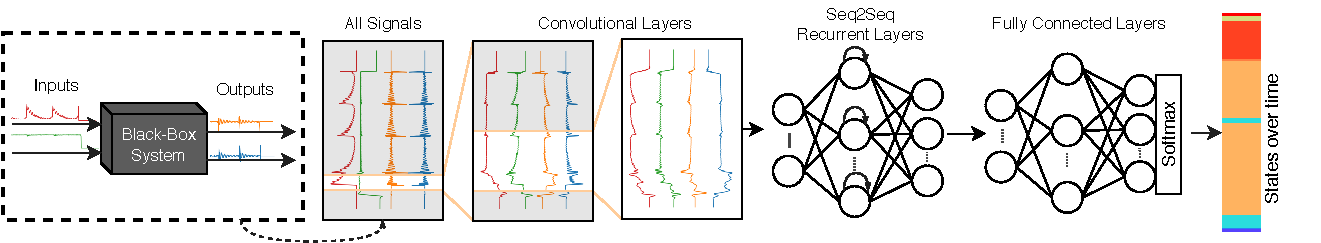
\includegraphics[width=\textwidth]{ASE_files/GeneralConvolutionalNet.pdf}
    \caption{The input and output signals of the black-box system are captured as a multivariate time series; they are processed in a deep neural network that consists of 3 sections: convolutional, recurrent, and dense (fully connected) to predict the system's internal state and its changes over time.}
    \label{fig:general_net}
\end{figure*}

The goal of this study is to infer the states of a running software system, over time. Given that my assumption is we don't have access to the source code (or part of it), I only leverage the values of inputs and outputs of the system, over time. 
As can be seen in figure~\ref{fig:general_net}, I capture all the inputs and outputs of the system as a time series and then process it in a DNN. 
The architecture of my proposed model is a hybrid DNN which is inspired by models proposed in the field of Human Activity Recognition (HAR). This task is quite similar to the subject of this thesis in the sense that they both take in a multivariate time series-data (from sensor readings) and output the state of the system that generated those readings (see section~\ref{sec:related_work_har} for more details on HAR papers). 
This DNN is made of three parts in sequence: 1) Convolutional, 2) Recurrent, and 3) Fully connected layers. This architecture addresses the aforementioned traditional methods' challenges; each part serves a different purpose in this process, as follows.


Convolutions, being more generalized than simple sliding windows, can discover patterns and features in the signals, both in temporal and in spatial (how signals affect each other) dimensions \cite{wang2017time}. 
The convolutional layers' flexibility allows them to learn some typical preprocessing operations. For example a moving average or a discrete derivative can be learned as simple convolutional filters. They also help the model to be more resilient to varying time delays between noticing a deviation in input signals and the reaction that will appear in the output signals. Applying convolutional layers in sequence has been shown to result in each layer learning more complex features than the previous layers \cite{zeiler2014visualizing}.
The number of layers, filters, and the kernel size are hyper-parameters that should be selected based on the size of data and the complexity of the system being modeled.
Using a sequence of convolutions with a) increasing number of filters and the same kernel size, b) same number of filters and increasing kernel size, and c) decreasing filters with increasing kernel sizes are all different approaches that have been used in the literature by well-known architectures such as VGG and U-net \cite{simonyan2014very, ronneberger2015u}. 
I will discuss more details of CNN layers in my approach in Section~\ref{sec:architecture_detail}.

Convolutions are quite powerful in discovering local features. To capture long-term features, recurrent layers which learn sequences of data are leveraged. For example, in my case, they can learn that ``accelerate'' and ``take off'' states only happen in the start of the states sequence, and each ``take off'' state is usually followed by a ``climb'' state. The type of recurrent cell to use (LSTM, GRU, etc.), how many cells to unravel in the layer, and the number of layers are also hyper-parameters that need to be tuned depending on the size and complexity of the system under study.

Finally, one or more dense (fully connected) layers in the end are a common way of reducing the dimensions to match expected output dimensions. 
If there are only two states, the last layer can have a sigmoid activation function and be of shape $L$ (the length of the input), otherwise, to match the one-hot encoding of labels, an output of shape $L\times N_s$ with softmax activation along the second axis ($N_s$) is required ($N_s$ being the number of possible states).

In terms of loss function to optimize in the training process, a good choice is a dice overlap loss function, which is used in image semantic segmentation tasks, as well. An important property of this loss function is not getting negatively affected by class imbalances \cite{milletari2016v, sudre2017generalised}.

% To make it more clear, compare it to applying a convolution (or a discrete derivative) to each signal independently. It can only learn temporal features, nothing about the interactions between the signals.
% Using convolutional layers instead of predefined kernels allows the model to learn which subset of possible connections and interactions (which can involve two or more variables) can be used as features. This flexibility has another advantage as well. It helps the model to be more resilient to time lag between noticing a deviation in input signals and the reaction that will appear in the output signals. This time lag can be caused by a number of reasons including: physical limitations, sampling resolution, tuning of the controller, or design choices in the system.
%\subsubsection{Data Collection}
%The object system is treated as a black-box where we can only read its input and output values. 
%Capturing the input and output data ($T_k$s) is straightforward. In the first step the system is executed and multiple logs of the input/output values are recorded. After that, state change points ($CP_k$s) data is required to be collected. A typical way to obtain them is with help of a domain expert. They label the logs indicating the time stamps where the system's internal state has changed as well as the new state that it went in. Domain experts are ideal for labeling since they know what the system is and what it is supposed to do, so they can (probably with some inherent human error) detect the system state. 
%They can do it based on a variety of information sources such as examining the system's I/O (which we already have captured), logs, or a high level program or set of instructions preloaded into the system.


%We aimed to infer high level states of a black-box system using a machine learning model that observes the system's behavior. 
\section{Data Encoding}
% To collect data we run the system $N$ times using $N$ existing test cases and record the input/output values. The recorded data from $k$-th run, $T_k$, forms a discrete multivariate time series data.
The input/output values of the black-box system create a multivariate time-series ($T_k$), which can be defined as a set of $n$ univariate time series ($V_i$) of the same length $l_k$. Each $V_i$ corresponds to the recorded values for one of the inputs or outputs of the system:
\begin{equation} \label{eq:T_k}
    T_k = \{{V_1}_k, {V_2}_k, \ldots, {V_n}_k\}
\end{equation}
\begin{equation} \label{eq:l_k}
    |{V_1}_k|=|{V_2}_k|=\ldots=|{V_n}_k|=l_k 
\end{equation}

Note that, as figure~\ref{fig:general_net} shows, we take both inputs and outputs as part of the time-series data to be fed as input into my deep learning models. 
This is to make sure that we can model state-based behavior of the system, where the current state depends not only on the inputs, but also on the last state(s) (captured as previous outputs) of the system. As an example, from the case study, if the outputs are not taken into account 
% the ``acceleration'' state before ``takeoff'' and the breaking state after landing
a mid-flight ``descend'' state and the ``approach'' state right before landing
are indistinguishable, using the sensor readings (inputs) alone. 

Having such a time-series, the only remaining pieces from a training set are the labels. Unlike the input/output values (the features in the data set) the labels are not usually given. My method to infer the labels is a supervised approach. Thus, we need the domain expert to manually label each individual time stamp with a state name/ID. In practice, what they would do is to identify the approximate time that a state change happens and assign the new state to one of the previous states labels or define a new label for this new state.
Thus I encode the states information over time as a set of tuples in the form of $(t_s, s)$ where $t_s$ denotes the timestamp where the system entered state $s$. We show the set of all possible states with $S$ ($s \in S$) and define $N_s$ as the cardinality of this set. 
\begin{equation}\label{eq:change_point}\begin{split}
    CP_k {}&{}= \big\{ (t_{s_1}, s_1), (t_{s_2}, s_2), \ldots, (t_{s_l}, s_l) \big\}\:,\; s_i \in S \\
    N_s  {}&{}= |S|
\end{split}
\end{equation}
So in summary, the dataset consists of $N$ pairs of the I/O values as features and their state information as labels $\big\{(X=T_k,\;y=CP_k)|1\leq~k\leq~N\big\}$. 
% Each example in dataset contains one whole test case. The output labels were one-hot encoded to match the model output shape.
%It is worth mentioning that in section~\ref{mp_data_collection} we explain what we did to keep the variety of the collected data (and hence its quality) high. 

\subsection{Data Preprocessing}
%\subsubsection{Inputs and Labels} %\label{data_set_properties}
Before being fed into the model $\mathcal{F}$ (as defined below), the inputs and labels need some preprocessing. 
\begin{equation}\label{eq:model_F}
    \mathcal{F}(\delta(T), m) \colon \mathbb{R}^{L\times n}\times\mathbb{R}^L\to S^{L}.
\end{equation}
To run more efficiently, TensorFlow expects all the inputs to have the same length. To do that, the shorter $T_k$s should be zero-padded to length $L = max\{l_k\}$. The padding function $\delta$ does that.
Therefore, eventually, the input to the model will be $T_k$s that are rearranged to form a tensor of shape $n \times L$ along with a padding mask (denoted with $m$). 
The mask tells the model where the tail starts so the model can ignore all the zeros from there on. % It prevents the added zero values to have a negative effect on the model's performance.
%The inputs are the sampled in/out values of the system given in form of $n$ time series of length $L$.
\begin{equation}\label{eq:model_as_function}
\begin{split}
    \hat{O} {}&{}= \langle \hat{o}_i \in S \rangle^L_{i=1} = \mathcal{F}\left(\left[ {\delta(V_1)}^\intercal \: {\delta(V_2)}^\intercal \; \ldots \; {\delta(V_n)}^\intercal \right],m\right) \\
    % \delta(V_i) {}&{}= \left[V_i \quad \vec{0}_{L-l}\right] \\
    m {}&{}= \delta(\vec{\mathds{1}}_l) \quad\text{i.e.}\quad \langle {m}_j \rangle^l_{j=1} = 1\:, \: \langle {m}_j \rangle^L_{j=l+1} = 0 \\
\end{split}
\end{equation}
Here $l$ denotes the length of the input before padding. It is equal to $l_k$ for the $k$th training data ($T_k$).


As defined in \eqref{eq:change_point}, $CP_k$s are tuples of $(t, s)$ which indicate the system have gone into state $s$ at time $t$. To train the model, $CP_k$ needs to be expanded into a vector of length $L$ denoted by $O$ where each element $o_t$ holds the state at time $t$. To define it formally, the elements can be derived from $CP_k$ using the following formula:
\begin{equation} \label{eq:output}
\begin{split}
O = \langle  \forall t \in \mathbb{N}_L : s_i \:|\:
           (& t_{s_i}, s_i) \in CP_k \: \land  \\
            & t_{s_i} = max\{t_{s_j} \:|\: (t_{s_j}, s_j) \in CP_k \land t_{s_j}\leq t\} \rangle
\end{split}
\end{equation}
For example: Suppose $L=10$ and $CP = \{(0, a),\:(3, b),\:(5, c),\:(8, a)\}$ 
% which means starting with state $a$ then going to state $b$ at time $t=3$,\ldots and it goes on for 10 steps; 
then $O = \langle a\:a\:a\:b\:b\:c\:c\:c\:a\:a \rangle$.
If there are more than two possible states ($N_s > 2$), $O$ needs to be one-hot encoded, at this stage.



\section{The Model Implementation} \label{sec:architecture_detail}
The first few layers of the model are convolutional layers. I used 5 convolutional layers with 64 filters each and a growing kernel size.
The intuition behind this design is that starting with a small kernel guides the training in a way that the first layers learn simpler more local features that fits in their window (kernel size).
Kernel sizes started with 3 since it is a common number in the literature for kernel sizes, then I used multiples of 5 from 5 to 20. 
The rationale behind choosing 5 is because the sampling frequency is 5, so each layer with a kernel size of $5n$ processes a whole $n$ seconds worth of simulation data, in each step.
Stopping at kernel size of 20 was a compromise between generalizability and model size. Generally, a larger model has more learning capacity, but it is also more prone to over-fitting. The current models are the smallest I could make the models (to avoid over-fitting), without compromising the performance.

Same compromise was made in the second section of the model (Recurrent layers), the sweet spot for hyper-parameters here was to use two GRU layers with 128 cells each. Their output was fed into a fully connected layer with 128 neurons with a leaky ReLU ($\alpha=0.3$) activation function \cite{maas2013rectifier} and finally to a dense layer with $N_s=25$ units with softmax activation.
I used Adam optimizer \cite{kingma2014adam} that could converge in 60-80 epochs, i.e. validation accuracy plateaued. The full architecture can be seen in figure~\ref{fig:model_arch}.
\begin{landscape}
\begin{figure*}
    \centering
    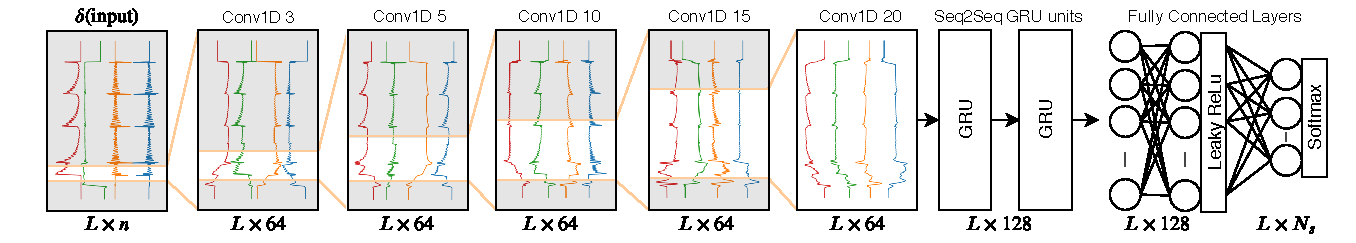
\includegraphics[width=\columnwidth]{ASE_files/Convolutional_Net.pdf}
    \caption{Model architecture in a nutshell. Tandem convolutional layers with increasing kernel size fed into two sequence-to-sequence recurrent layers with 128 GRU cells each, which is then fed into dense layers to output the predicted system state, as a list of one-hot encoded states. $\hat{O}$ will be the result of applying argmax operation on the last layer's output. $L=18000,\: N_s=25$}
    \label{fig:model_arch}
\end{figure*}
\end{landscape}

\chapter{Empirical Evaluation} \label{sec:experiment}
%In this section we reiterate the problem, provide more detail about the experiment and evaluation process, and describe the system and the data we collected from it to perform the study.
In this section, I explain my empirical evaluation process of the proposed approach through two case studies.

\section{The Study Objectives}
The goals of this study is to evaluate our proposed method in terms of change point detection and state inference, in comparison to traditional techniques in this domain.  Therefore, our research questions are as follows:

\subsection{RQ 1) How does our proposed technique perform in detecting the state changes?}
The goal of this RQ is to see how close the predicted state-change times are to the real state-change times.  In other words, in RQ1, we do not predict the exact state labels and are only interested in predicting the change.
To answer this question, we compare the performance of our proposed approach with several traditional baselines (see \ref{sec:CPD_baseline}), in terms of modified precision, recall, and F1 scores that are introduced in section \ref{sec:CPD_metrics}.


\subsection{RQ 2) How well does our proposed technique predict the internal state of the system?}
In RQ1, we are only interested in detecting the time a state-change happens (binary classification), but here in RQ2, we extend that and are also interested in predicting the label of the new state that the system is going into (multi-class classification).  
%We need to evaluate how similar is our model's prediction about the internal state of the system at each time $t$ to the actual state.
Therefore, to answer this RQ, we change the labels from a Boolean (changed/not changed) to the actual collected labels. 

\subsection{RQ 3) Can the results be replicated with regards to state change point detection (RQ1) on Paparazzi auto pilot?}
\hl{In the first two research question, I evaluate my proposed model inference technique on the data collected from our industry partner, MicroPilot. However, to confirm the results and idea furthermore, a replication on a similar software is quite helpful. 
In this RQ and the next one I want to explore how my method performs on Paparazzi, an open source equivalent to MP\footnote{MicroPilot}'s auto pilot.}

% I chose Paparazzi auto pilot as an open source alternative to MP's auto-pilot for replication. 
Paparazzi \cite{hattenberger2014using} project started in 2003 as an academic auto-pilot and continues to be developed with the state of the art in the autonomous flying vehicle's field. Another major player in open source auto-pilot software scene is ArduPlane; however I chose to do this study only on Paparazzi for the following reasons:
A comparison about how Paparazzi is superior to ArduPlane can be read at \url{https://wiki.paparazziuav.org/wiki/Paparazzi_vs_X}. 
In addition to that, after doing a preliminary study, I found out that Paparazzi has a more straightforward and robust protocol for remote controlling and data collection, as explained previously in section~\ref{sec:paparazzi_data_collection}. 
Furthermore, Paparazzi supports multiple flight dynamic model (FDM) simulators. One of them is JBSim\footnote{\url{http://jsbsim.sourceforge.net/}} which provides an advanced physical model of complex dynamics in air-frames and sensors for an accurate and close to the reality simulation. 



\subsection{RQ 4) Can the results of internal state prediction task (RQ2) be replicated on Paparazzi auto pilot?}
\hl{I fed the data to a number of classic machine learning algorithms as baselines. The problem setting is a multi-class classification, though with Paparazzi the number of classes are smaller. 
There are 20 possible states in Paparazzi as opposed to MicroPilot's 25. This is due to their differences in solving the problem of defining a mission and controlling an automated vehicle (the aircraft) to perform it.}

\subsection{RQ 5) How will hyper-parameter tuning affect the results?}
\hl{In RQs 1 and 2 the hyper-parameters of the neural network model are tuned manually. Hyper-parameters include the number of convolutional layers, number of convolutional filters in each layer, number of recurrent cells, and optimizer parameters such as learning rate. There are no gold standards for the values of these parameters, they need to be tuned for each problem. In the replication (RQs 3 and 4) I opted for existing automated ways for finding better hyper-parameters.}

I created a model creation and evaluation pipeline that takes hyper-parameters as the input and outputs the model performance scores on test data as its output. The hyper-parameters that I searched over are:
\begin{itemize}
    \item Number of GRU cells in the recurrent section: between 32 and 256
    \item Number of convolutional filters in each layer: between 16 to 64
    \item The size of convolution kernels and the number of convolutional layers: between 3 to 5 layers with increasing kernel size
    \item The learning rate of Adam optimizer: from $1\times 10^{-4}$ to $3\times10^{-3}$
\end{itemize}
Please refer to figure~\ref{fig:model_arch} for a recap on these hyper-parameters. 
I performed an exhaustive grid search over these parameters, using Tensor Board for keeping track of the metrics and finding the right balance.
Tensor Board is a monitoring tool made for TensorFlow \cite{tensorflow2015-whitepaper} that provides great insight for better training TensorFlow models.


Note that in our empirical study to evaluate our approach, we use the source code to collect the exact time a state-change happens and the actual state labels (ground truth). However, in practice, labeling the training set is supposed to be done by the domain expert in a black-box manner. This is not an infeasible task or extra overhead. Monitoring the logs and identifying the current system state is in fact part of the developers/testers regular practice during inspection and debugging. All we provide here is a tool that given a partial labeling (only on the training set), automatically predict the state labels and the state-change times, for future flights.  Also note that even though we use the source code to label the training set, we still look at the test set as a black-box and don't leak any information.

\section{Evaluation Metrics}
\subsection{CPD Performance Metrics (RQs 1,3, and 5)} \label{sec:CPD_metrics}
%In CPD-natured tasks 
Given that in RQ1 there is an inherent class imbalance (there are far more points where a change has \textit{not} happened compared to points with a state-change positive label), we avoid using accuracy and report both precision and recall. %, so the sheer number of true negatives makes metrics such as accuracy almost useless. A trivial model can always output 0 (no change) and have an accuracy of 99\% on a input of length 1000 with 10 true change points.To address this problem, metrics such as precision and recall that do not account for true negatives are used in the literature \cite{Truong2018ChangePointSurvey, Lee2018TimeSeriesSegmentation}.
However, the original precision/recall metrics require some modifications due to the difficulty of predicting the exact time stamp that a state-change happened. To handle this, similar to related work \cite{Truong2018ChangePointSurvey}, we use a tolerance margin $\tau$. If a detected state-change ($\in\hat{CP}_k$) is within $\pm\tau$ of a true change ($\in{CP}_k$) , we call the prediction a True Positive, otherwise it is a False Positive. Similar adjustment to definition is applied for True Negative and False Negative. 
Formally speaking, we define predicted change points for $k$-th sample as:
\begin{equation} \label{eq:cp_hat}
\hat{CP}_k = \big\{(t, \hat{o}_t)\: |\: \hat{o}_t \neq \hat{o}_{t-1} \big\}
\end{equation}
Please note that in \eqref{eq:cp_hat}, $\hat{o}_t$ refers to $t$-th element of output vector $\hat{O}$, as previously defined in \eqref{eq:model_as_function}. Based on that the confusion matrix elements are calculated as:
\begin{equation} \label{eq:metrics}
\begin{split}
TP ={}&{}\Big|\big\{ (\hat{t}, \hat{s}_t) \in \hat{CP}_k \;\big|\; \exists\: (t, s_t) \in CP_k \;\text{s.t.}\; |t - \hat{t}| < \tau\big\}\Big| \\
FP ={}&{}\Big|\big\{ (\hat{t}, \hat{s}_t) \in \hat{CP}_k \;\big|\; \nexists\: (t, s_t) \in CP_k \;\text{s.t.}\; |t - \hat{t}| < \tau\big\}\Big| \\
FN ={}&{}\Big|\big\{ (t, s_t) \in CP_k \;\big|\; \nexists\: (\hat{t}, \hat{s}_t) \in \hat{CP}_k \;\text{s.t.}\; |t - \hat{t}| < \tau\big\}\Big| 
\end{split}
\end{equation}
With these in mind, we measure precision, recall, and their harmonic mean F1 Score with three values for $\tau$: 1, 3, and 5 seconds. The smaller the tolerance is the stricter the definitions become and the lower the numbers are. 

\subsection{State detection metrics (RQs 2, 4, and 5)}
% To answer RQ2, we again use the modified confusion matrix (using the tolerance margin $\tau$), but  
In RQ2, we have a multi-class classification problem and thus multiple precisions/recalls will be calculated, one per class (state label). We then report the mean value across all classes. 
\begin{equation}
\begin{split}
P_s ={}&{}\big\{\hat{s}_t \in \hat{O}_k \;\big|\; \hat{s}_t = s\big\} \\
T_s ={}&{}\big\{s_t \in O_k \;\big|\; s_t = s\big\} \\
TP_s ={}&{}\big\{\hat{s}_t \in P_s \;\big|\; \hat{s}_t = s_t \in O_k\big\} \\
\end{split}
\end{equation}
$$Precision =\frac{1}{N_s}\sum_{s=1}^{N_s} \frac{|TP_s|}{|P_s|} \quad,\quad Recall = \frac{1}{N_s}\sum_{s=1}^{N_s} \frac{|TP_s|}{|T_s|}$$

\section{Comparison Baselines} 
\subsection{CPD baselines (RQs 1 and 3)} \label{sec:CPD_baseline}
We used `ruptures' library developed by authors of a recent CPD survey study \cite{Truong2018ChangePointSurvey}. It provides a modular framework for applying several CPD algorithms to univariate and multivariate data. % We did not apply the methods that required knowing the number of change points a priori. 
As mentioned earlier two main elements of a CPD algorithm in their survey are the search method and the cost function.

I used Pelt \cite{killick2012optimal} as the most efficient exact search method. As examples of approximate search methods, we applied bottom-up segmentation and window-based methods using a default window size of 100 \cite{keogh2001online}.
However, after trying to run Pelt algorithm \hl{on MicroPilot's data}, we realized that it takes prohibitively longer to run compared to the approximate methods without providing much better results, so we only use the bottom-up and the window-based segmentation methods, as our CPD baselines in RQ1.
\hl{Fortunately, for RQ 3 with smaller data set size of Papaarazzi, it was feasible (though still quite time-consuming) to try ``Pelt'' as well, making the replication question richer in that sense.}

For the cost function, I tried ``Least Absolute Deviation'', ``Least Squared Deviation'', ``Gaussian Process Change'', ``Kernelized Mean Change'', ``Linear Model Change'', ``Rank-based Cost Function'', and ``Auto-regressive model change'' as defined in the library. Their parameters were left as default.
To optimize the number of change points a penalty value (linearly proportionate to the number of detected change points) is added to the cost function, which limits the number of detected change points, the higher the penalty the fewer reported change points. We tried three different ratios (100, 500, and 1000) for the penalty.

\subsection{Multi-class classification baselines (RQs 2 and 4)}
We used a sliding window of width $w$ over the 10 time-series values and then flattened it to make a vector of size $10w$ as the features. For the labels, we used one-hot encoded state of the system.
The window sizes were chosen as same as the sizes of convolutional layers' kernel sizes (3, 5, 10, 15, 20), to make the baselines better comparable with our method. 
We used Scikit-learn's implementation of the classification algorithms: A ridge classifier (Logistic regression with L2 regularization) and three decision trees. The ridge classifier was configured to use the built-in cross validation to automatically chose the best regularization hyper-parameter $\alpha$ in the range of $10^{-6}$ to $10^6$. Each decision tree was regularized by setting ``maximum number of features'' and ``maximum depth''. For ``maximum number of features'' we tried no limits, $\sqrt{10w}$, and $\log_2{10w}$. To find best ``maximum depth'' we first tried having no upper bound and observed how deep the tree grows; then we tried multiple numbers less than the maximum, until a drop in performance was observed. 

\hl{In RQ4, pretty similar to RQ2,} I used a ridge classifier and a decision tree classifier with 3 settings for maximum number of features with no limit on their depths. This setting is the same as the MP's case (RQ2), with the only difference being on removing the depth limit. Tuning the depth limit was an arduous and inaccurate task that resulted in minimal improvements (if any, as will be seen in the RQ2's answer later on), so it was not worth the time. Overall, I ran $(1+3)\times6=24$ different settings for classic learning algorithms to answer RQ4. 






\section{Data Collection Process}
In this section more details on how data was collected from each system will be presented. 

\subsection{MicroPilot AutoPilot}
\subsubsection{Instrumentation}
Control decisions in this software are made in a 5Hz loop, it means that every 200ms all the sensor inputs are read and based on the current state of the aircraft and the system's goal at the moment (e.g. maintaining a constant speed) decisions will be made and output is generated. Considering this, the best way to capture those data is in the end of each iteration of this loop. I inserted instrumentation code there, to log input and output values (listed in Table~\ref{tab:in_outs}) at the exact spot where they are updated. 
Please note that although it is more convenient to capture the values in this way, it does not give us any special advantage or insight that breaks the black-box condition. In other words, the exact same data could be collected from the compiled binaries without any access to the internals, just with extra steps. Inputs and outputs, after all, are the very least thing available in both black-box and white-box settings.

\subsubsection{Test Scenarios}\label{sec:mp_test_scenarios}
MicroPilot has a repository of 948 system tests, I ran them in a software simulator\footnote{It is developed by MicroPilot and provides an accurate simulation of the aerodynamic forces on the aircraft, the physical environment irregularities (e.g. unexpected wind gusts), and noises in sensor readings} and collected the logged flight data, over time. 
The test cases are system-level tests. Each test case includes a flight scenario for various supported aircraft. A flight scenario goes through different phases in a flight such as ``take off'', ``climb'', ``cruise'', ``hitting way points'', and ``landing''.
\begin{table}
    \caption{The $n=10$ collected I/Os of AutoPilot. The inputs are sensor readings and the outputs are the servo position update commands. All these I/Os over time are used as the inputs of the state prediction model.}
    \label{tab:in_outs}
    \centering
\begin{tabularx}{\columnwidth}{lX}
                                                                                                                    \toprule
\multicolumn{2}{l}{\textbf{Inputs}}                                                                              \\ \midrule
Pitch     & The angle that aircraft's nose makes with the horizon around lateral axis                            \\ 
Roll      & The angle of aircraft's wings make with the horizon around longitudinal axis                         \\ 
Yaw       & The rotation angle of aircraft around the vertical axis                                              \\ 
Altitude  & AGL\footnotemark Altitude                                                                            \\ 
Air speed & Speed of the aircraft relative to the air                                                            \\ \midrule
\multicolumn{2}{l}{\textbf{Outputs}}                                                                             \\ \midrule
Elevator  & Control surfaces that control the Pitch                                                              \\ 
Aileron   & Control surfaces that control the Roll                                                               \\ 
Rudder    & Control surface that controls the Yaw                                                                \\ 
Throttle  & Controller of engine's power, ranges from 0 to 1                                                     \\ 
Flaps     & Surfaces of back of the wings that provide extra lift at low speeds, usually used during the landing \\ \bottomrule
\end{tabularx}
\end{table}
\footnotetext{Above Ground Level}
Out of the 948 flight logs, I omitted 60 that were either too short or too long (shorter than 200 samples or longer than 20k samples). Figure~\ref{fig:test_lengths} shows the distribution of the remaining log lengths. The maximum length ($L$) was 18,000 samples.

\begin{figure}
    \centering
    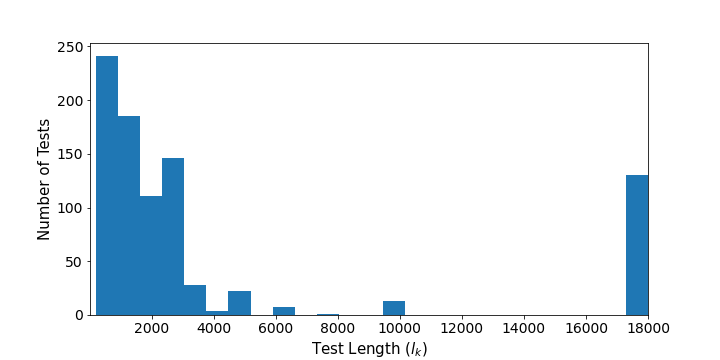
\includegraphics[width=\columnwidth]{ASE_files/test_lengths.png}
    % \Description[Number of tests histogram]{A histogram chart maxing on numbers less than 2,000 and over 17,500}
    \caption{Distribution of flight log lengths for the $N=888$ (out of the original 948 available logs) logs that were kept in the dataset ($200 \leq l_k \leq 20,000$), \hl{from MicroPilot.}}
    \label{fig:test_lengths}
\end{figure}

% As mentioned before each input data item is a multivariate time series with $n=10$ variables (listed in table~\ref{tab:in_outs}). 
% During the data preprocessing, after the time series data is converted into tensors, all of the shorter $T_i$s were post-padded to the length of the longest one: $L=18000$ time steps.
The dataset was randomly split into three chunks of 90\%, 5\%, and 5\% for training, validation, and testing, where each sample corresponds to one test execution. Note that separate test and validation sets are needed to facilitate proper hyper-parameters tuning, without leaking information. 
% \subsection{System Under Study} \label{mp_data_collection}
% Our case study is a state-based system, which is real-time controller for UAVs, developed by
% our partner
% \begin{anonsuppress}
% Winnipeg based Micropilot Inc. Micropilot is the world-leader in professional UAV AutoPilot which develops both hardware and software for 1000+ clients (including NASA, Raytheon, and Northrop Grumman) in 85+ countries during the past 20+ years.
% \end{anonsuppress}
% .

%What the AutoPilot does can be summarized as `trying to hold some invariants based on the goal/state of the system'.
% % Maybe these two paragraphs can be moved somewhere more appropriate
% \label{changes_in_inputs}
% To work it backwards we capture the input/outputs (the UAV's relevant signals) over time and examine their correlations, i.e. how changes in one of them results in changes in another. When the state of the system changes these relations may change. So if we can capture what the relations are and when they change we can determine the state in which the system is in. 
% Of course pinpointing the exact moment when the changes happen is difficult; It is also impacted by the sampling time resolution so the inferred states and the change points are approximations.
The auto pilot can be used in SWIL and HWIL modes \cite{melmoth2019true}, which stand for software in the loop and hardware in the loop respectively. I used SWIL mode as it provides what was needed without any of the costs and hassles that come from HWIL mode. 

\subsection{Paparazzi}\label{sec:paparazzi_data_collection}

\hl{This sub section is new}

\subsubsection{Instrumentation}
Paparazzi provides a rich and flexible API that can be configured to record several different parameters in flight. The aircraft periodically sends data back to the ground station over a wireless link using a protocol called Paparazzi link. Paparazzi link is built over Ivy, a message bus protocol that uses UDP. 
In Paparazzi's architecture a process called `link' interfaces the wireless link to the aircraft to the computer's network; on one side are the Paparazzi link messages that come and go as UDP datagrams and on its other side is the (often wireless\footnote{A wired connection is used in HWIL test mode as well as some scenarios where the AutoPilot equipment is used in a autonomous submarine rather than an autonomous unmanned aircraft.}) connection to the aircraft.
In simulations, the modem and wireless communications are no longer needed, instead the auto pilot runs as a separate process and mimics a wireless channel over the local network. (See Figure~\ref{fig:paparazzi_comm_agents})

\begin{figure}
    \centering
    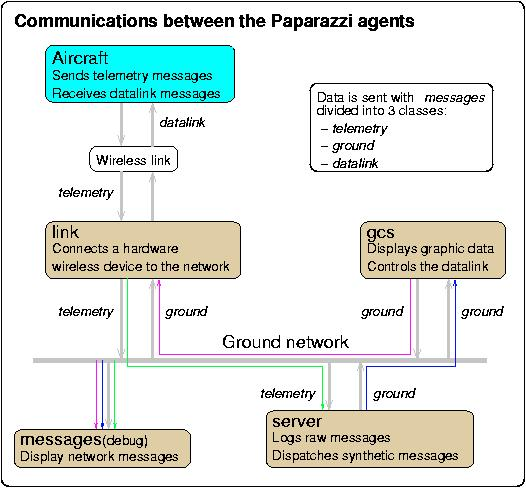
\includegraphics[width=\columnwidth]{4_files/Pprz_communication_agents.jpg}
    \caption{High level overview of communication links architecture in Paparazzi \cite{hattenberger2014using}}
    \label{fig:paparazzi_comm_agents}
\end{figure}

Paparazzi comes with a multitude of small tools that could do most of what I needed in terms of instrumentation. There is a remote logger and a log player which are quite close to the instrumentation tool I need, however upon trying them in action, I figured that they cannot record some of the information that I need. Therefore, I developed a custom flight data recorder tool. 

\subsubsection{Test Scenarios}
Unlike MicroPilot that had a quite a number of system tests (in addition to other types of tests such as unit tests which I did not use), Paparazzi comes with only unit tests. As it is an open source software under GPL licence it comes with no warranty and also does not need certain certifications and approvals that commercial systems require, therefore incentives to have such tests are lower. 
Although it is a reliable and widely used auto pilot, it owes that reliability more to its widespread use in action (by many researchers and enthusiasts) rather than automated tests that verify its behaviour.
In this situation, where many eyes are watching over the code, bugs are discovered and patched quickly. However, to the best of my knowledge they are not recorded as system tests that verify the bugs are properly patched and detect regressions in the future.

To fill the void, I created a fuzz testing tool that can automatically generate valid, diverse, and meaningful automated system tests for Paparazzi based on the example flight plan that is included with it.
My tool can automatically generate system tests, run them in a simulator (or on hardware\footnote{Although I have not tested running tests on a hardware (HWIL) to confirm, but having implemented the protocol it potentially is capable of doing so}), and also collect required telemetry data from the aircraft. 
%run them automatically, and integrated it with the flight data recorder tool to generate the data set for downstream tasks. 
It is called PprzTester and the source code, version history, project planning data (bugs, enhancements, tasks and issues, etc), and the documentations are available on GitHub at \url{https://github.com/MJafarMashhadi/pprz_tester}. 
The targeted randomizations in test inputs are augmented with the stochastic wind model in the simulation to further diversify the observed behaviours.

In addition to that tool, I needed to patch some parts of Paparazzi to make the logging and testing more similar to MicroPilot, for example increase telemetry reporting rate from 2Hz to 5Hz. A list of these patches including the reason why that change was necessary or beneficial and the exact lines of code that need to be changed is available in the project wiki at \url{https://github.com/MJafarMashhadi/pprz_tester/wiki/Paparazzi-Patches}.
Aside from the patches, I found some bugs, missing features, missing documentations, and bad smells in the code that needed to be fixed. I contributed new code and documentation to the Paparazzi project to address these issues. The contributions were useful, up to the standards, and welcome in the project; they are included in the latest release\footnote{as of August 3rd, 2020} of Paparazzi auto pilot: version 5.16.

More details about the tool is left for next section, section~\ref{section:fuzzing_tool}.
The result of generating and running tests was 378 runs worth of different flight scenarios.
After collecting the data I performed some pre-processing steps on them to make them more similar to what the previous model was trained on. These pre-processing steps include normalizing some values as well as metric to imperial unit conversions.

Figure~\ref{fig:paparazzi_test_length} shows the distribution of the test lengths. The test lengths range from 140 samples (70 seconds) to 2580 samples, with a median of 2170 and a mean of 1896.
\begin{figure}
    \centering
    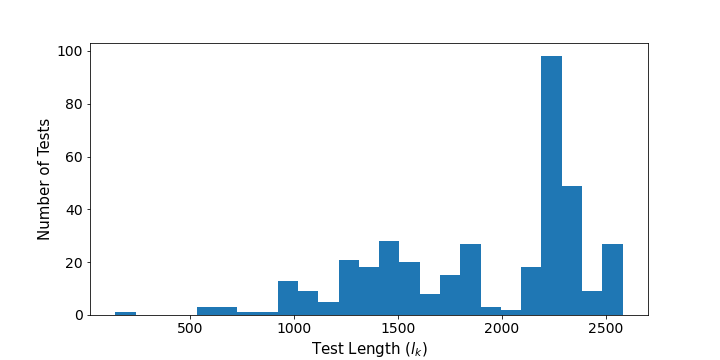
\includegraphics[width=\columnwidth]{6_files/test_lengths.png}
    \caption{The histogram of number of tests of different test sizes. The smallest samples contains 140 samples worth of recorded flight data and the largest one has 2580 samples, equivalent of a 516-second flight (Sampling rate is 5Hz). }
    \label{fig:paparazzi_test_length}
\end{figure}

The training data was split into 3 chunks after shuffling: 70\% of the data was used for training, 20\% was used as the test set for tuning the hyper-parameters, and the remaining 10\% was set aside as the validation data to measure the trained model's performance. 







\subsection{The Testing and Data Processing Tool Set}\label{section:fuzzing_tool}
I implemented the pipeline of generating tests, running them, and aggregating flight logs in an integrated tool with three components, one for each stage. In the following sections I will explain these components and their role in the system. I also very briefly explain how event-driven programming paradigm was implemented here both to decrease coupling and to make it more resilient to unexpected or buggy behaviour. It is necessary for two reasons: 1. as a testing tool, it is \textit{expected} to encounter bugs in software under test and should be resilient to them 2. the message passing design of Paparazzi architecture, in addition to its ability to support multiple aircraft in flight at the same time left me with no choice but to use an event-driven design.


\subsubsection{Flight Data Recorder}
Although Paparazzi comes with a logging feature in its `server' component (Figure~\ref{fig:paparazzi_comm_agents}), it only logs a subset of required data. Furthermore, the data comes in separate messages with different frequencies; for example speed updates are sent in \verb|AIRSPEED| message once a second, orientation updates and engine rpm are reported in \verb|ATTITUDE| and \verb|ENGINE_STATUS| messages respectively which are dispatched every 200 milliseconds, while servo outputs are only sent once every 5 seconds. All these data need to be aggregated and aligned. Please refer to the Table~\ref{tab:pprz_messages} in \hyperref[appendixa]{Appendix~A} for a full list of messages used.

The most flexible option with the least overhead is to have an independent module that understands Paparazzi link, captures these messages and does data aggregation and logging in real-time. So I created a flight data recorder to collect all the required data from telemetry messages.

In the beginning the instance of ``AircraftManager'' singleton class starts with listening for \verb|NEW_AIRCRAFT| messages. This message type notifies this class when new aircraft come online in the simulation. Then it sends a \verb|AIRCRAFTS_REQ| request message to server to get a list of currently online aircraft. The response to both of these messages are processed in the same way: The aircraft unique ID will be checked against the hash table of known aircraft, if it is a new one an ``Aircraft'' instance will be created and added to the hash table. (See the class diagram in Figure~\ref{fig:fdr_class_diagram} in \hyperref[appendixa]{Appendix~A})

Each ``Aircraft'' object in the makes a number of requests back and forth with other components in the system (server, data link, and the auto pilot process) to gather required information about that aircraft, including its flight plan. This class along with ``Aircraft Parameters'' and ``Aircraft Commands'' provide a unified programmatic API for monitoring and controlling the aircraft. 

I implemented observer pattern \cite{gamma1995design} in ``Aircraft Parameters'' to enable other components (such as flight data recorder and automated test executor) to listen for changes in the aircraft state and respond accordingly in an event-driven manner. 
After creation of an ``Aircraft'' object, as a part of its initialization, several observers are created and attached to it. A ``Record Flight'' instance is one of them. It observes new \verb|FLIGHT_PARAM| messages as well as changes in `throttle', `flight time', and `commands.values' parameters. This class stores and aligns these parameters in a pandas data frame which is stored on disk periodically. The data can be stored in a human-readable CSV file or as a compressed HD5 binary. Some data normalization and unit conversions (such as meters to feet) also happen before saving in order to make the generated data similar to MicroPilot's.

Supplementary UML diagrams are provided in \hyperref[appendixa]{Appendix~A}.


\subsubsection{Automated Test Executor}
Here I first explain how the test executor work, since knowing this is prerequisite of understanding the test generator component.
The test executor takes the control of the aircraft by running prefabricated test scenarios. While the low level control of the aircraft is done by the auto-pilot software (the system under test), it needs high level commands such as ``climb to 200ft''. Automated test executor does that, using hand crafted test scenarios or the ones generated by the test generator component.

Tests scenarios are defined as subclasses of \verb|PlanBase| class. Each plan needs to override a method that returns an iterable of plan items which should be executed one by one. 
\begin{lstlisting}[language=Python, basicstyle=\linespread{0.1}]
class ExamplePlan(PlanBase):
  def get_items(self, **kwargs):
    block_name = kwargs.pop('block_name')
    circles = int(kwargs.pop('circles'))
    return [items.JumpToBlock(block_name),
      items.WaitForCircles(n_circles=circles)]
\end{lstlisting}
The above plan for example, takes a block name and a number of circles as its parameter and executes the two items in succession. An example of running this plan can be like the command below:
\begin{lstlisting}[language=bash]
$ run_test.py ExampleAircraft ExamplePlan\ 
    -Dblock_name='loiter' -Dcircles=2
\end{lstlisting}
Using this parameters is analogous to test parameterization in mature unit testing frameworks (such as pytest). It allows similar test plans that are only different in some parameters to be consolidated in one test case.
Using parameters also improves the reproducibility of test scenarios while improving its flexibility. Test scenarios (plans) do not need to include commands for waiting for aircraft to take off and land, the testing tool automatically wraps it with appropriate initialization code.

The core test plan runner is implemented as an observer class that listens for multiple messages and parameters to get notified about changes in the aircraft's state (See Figure~\ref{fig:flight_plan_executor_class_diagram} in \hyperref[appendixa]{Appendix~A}). It iterates over the flight plan items and calls their \verb|match| method to decide whether that item should be executed. Whenever a match is found the item will be executed and the iterator will move to the next test plan item. Consult Figure~\ref{fig:flight_plan_items_class_diagram} in \hyperref[appendixa]{Appendix~A} for a class diagram of all flight plan items.

Test plans should be importable from \verb|pprz_tester.generated_plans| module. The structure is simple and clearly defined so that they can easily be handcrafted (like the example above) or generated using the test generator component.

The test runner is tailored specifically for Paparazzi in several ways:
\begin{enumerate}
    \item % First, 
As mentioned before, it takes care of aircraft initialization, take off, and landing
    \item %Second, 
It uses standard Paparazzi environment variables such as \verb|$PAPARAZZI_HOME|.\footnote{If it is not set, the user can use \texttt{-p /path/to/paprazzi} command line argument to set this value, and if that is not set too, a default value will be used.} 
    \item %Third, 
It can build the auto pilot if \verb|--build| argument is set so the user does not have to build it manually in Paprazzi center. 

    \item %Fourth, 
If \verb|--gcs| argument is set, the ground control station window will be opened (See Figure~\ref{fig:paparazzi_gcs}). It provides a real-time map that visualizes the aircraft path, waypoint locations, wind direction and velocity, and several other parameters of the aircraft such as their airspeed and altitude. 
    \item %And last, 
\verb|--no-sim| argument tells tester to not launch the simulator. Its use case can be when a physical auto pilot is being used (similar to MicroPilot's HWIL mode), or when for any reason the user chooses to run the simulator manually. 
\end{enumerate}

\begin{figure}
    \centering
    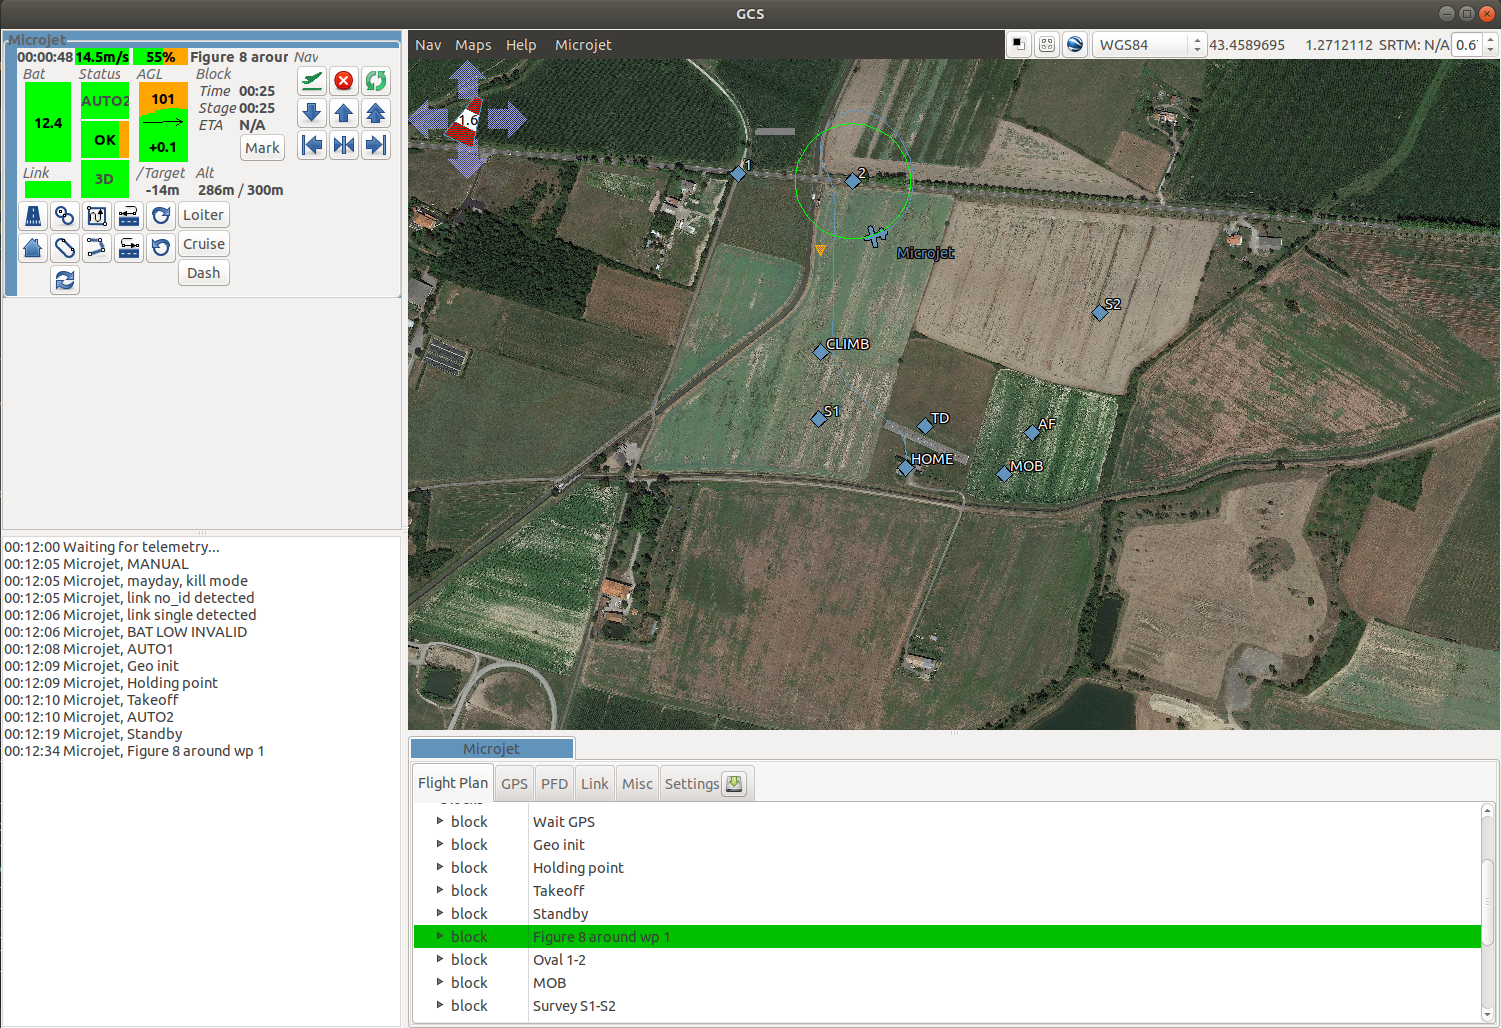
\includegraphics[width=\textwidth]{4_files/GCS.png}
    \caption{A snapshot of ground control station software (GCS), visualizing the map, waypoints (blue diamonds), the aircraft, its flight history (blue), the intended flight path (green), as well as its state (bottom in green) and some telemetry data (top left). The plan that it is following is one of the automatically generated test scenarios.}
    \label{fig:paparazzi_gcs}
\end{figure}

Test runner can move waypoints as well. The user can fix any number of waypoints at specified locations, providing their latitude longitude and altitudes. It can also randomize their location inside a cube. Boundaries of that cube (i.e. east-west, north-south, and floor-ceiling) are customizable through provided command line arguments.

The comprehensive list of command line arguments is included in Table~\ref{tab:test_runner_commandline_args} in \hyperref[appendixa]{Appendix~A}.


\subsubsection{Automated Test Generator}
The test generator component is a fuzz test generator specifically designed for Paparazzi. An auto pilot has plenty of parameters to change. Many of them need to remain unchanged. For example, changing aerodynamic and physical parameters of an air frame will make it behave incorrectly or even crash. A naïve algorithm might be tempted to only change these parameters to optimize a metric of ``bug''s per test. To comply with the constraints in input format and range and optimize test scenario diversity without having to have thousands of tests, I opted for developing a specialized automated test generator. 

This test generator is completely compatible with Paparazzi and designed with specific needs of an auto pilot in mind. It begins with loading and parsing the one fixed wing flight plan that comes with Paparazzi. It defines multiple actions (control blocks) available to a fixed wing aircraft. Two important components in the flight plan that are used are the waypoint names and locations, and available blocks. A test scenario is generated by taking the initial flight plan and fuzzing three parameters about it:
\begin{enumerate}
    \item Waypoint locations
    \item Sequence of actions 
    \item Action timing
\end{enumerate}

The test generator can be configured to fuzz all or some of them. \hl{I generated 31 tests with fuzzing the last two. Please note that the sequence of actions can have any length between 1 and the number of possible actions (5, in my case). Also for each sequence, $n!$ different permutations can be made that will result in very different outcomes. That makes the number of tests, $5!\times1+4!\times5+3!\times10+2!\times10+1!\times5=325$. Also note that these generated tests are made of unique blocks, in other words, a test scenario does not contain plans like ``Do A then B then A again'' while these plans are perfectly valid. In case one wants to have such plans they can write test plans manually.} \hl{to move}

The output is a python module that contains a subclass of \verb|PlanBase|, as expected by the automated test executor. These two work together seamlessly and the user can just use them in a plug-and-play manner without touching the code. Though, the generated code is designed to be effortlessly understandable and easily editable it even incorporates some auto-generated comments in the code.

The full table of command line arguments that test generator accepts is presented in Table~\ref{tab:test_generator_commandline_args} in \hyperref[appendixa]{Appendix~A}. To provide an example, the following command generates tests of length (number of actions) 2 for `Microjet' aircraft and writes it to the file \verb|l2.py| in the specified directory. It fuzzes the location (latitude, longitude, and altitude) of waypoint `S2' in the default cube, just overriding the altitude bounds in 200 to 220 meters, while the coordinates of `S1' are fixed. The initialization and landing stages which must be excluded from the test scenario are also specified. 
\begin{lstlisting}[language=bash]
gen_test.py --exclude "Wait GPS" "Geo init" "Holding 
point" Takeoff Standby "Land Right AF-TD" "Land Left 
AF-TD" land final flare --fuzz-wps S2 \
--wp-fuzz-bounds-alt 200 220 -w S1 43.4659053 1.27 300 \
--length 2 Microjet pprz_tester/generated_plans/l2.py
\end{lstlisting}
Some of the available actions and all the waypoints in this flight plan can be seen in Figure~\ref{fig:paparazzi_gcs}.













\section{Experiment Execution Environment} \label{sec:machines_config}
Training and evaluation of the deep learning model was done on a single node running Ubuntu 18.04 LTS (Linux 5.3.0) equipped with Intel Core i7-9700 CPU, 32 gigabytes of main memory, and 8 gigabytes of GPU memory on a NVIDIA GeForce RTX 2080 graphics card.
The code was implemented using keras on TensorFlow 2.0.

The baseline models could not fit on that machine, so two nodes on Compute Canada's Beluga cluster, one with 6 CPUs and 75GiB of memory and one with 16 CPUs and 64GiB of memory, were used to train and evaluate them.


\section{Results} \label{sec:results}
In this section, we present the results of the experiments and answer the two research questions. 
\subsection{RQ1 Results: CPD Performance}
\begin{sidewaystable} 
% \begin{table*}
\caption{Change point detection precision, recall, and F1-score calculated for the baseline methods using three values of tolerance ($\tau$) for multiple configurations.}
\label{tab:rq1-results}
\resizebox{\columnwidth}{!}{%
\begin{tabular}{llcccccccccc}
\toprule
  \textbf{Cost Function} &
  \textbf{Search Method} &
  \textbf{Penalty} &
  \textbf{Prec.} &
  \textbf{Recall} &
  \textbf{F1} &
  \textbf{Prec.} &
  \textbf{Recall} &
  \textbf{F1} &
  \textbf{Prec.} &
  \textbf{Recall} &
  \textbf{F1} \\
                                                  &              &   & \multicolumn{3}{c}{$\tau=1$s} & \multicolumn{3}{c}{$\tau=3$s} & \multicolumn{3}{c}{$\tau=5$s} \\  \toprule
\multirow{2}{*}{\textbf{Autoregressive Model}}     & Bottom Up    & 1000 & 10.43\%    & 75.44\%    & 18.33\%   & 21.21\%    & 80.32\%    & 33.55\%   & 28.94\%    & 81.22\%    & 42.68\%   \\
                                                   & Window Based & 100  & 2.94\%     & 3.98\%     & 3.38\%    & 8.53\%     & 11.41\%    & 9.76\%    & 12.89\%    & 17.54\%    & 14.86\%   \\ \midrule
\multirow{2}{*}{\textbf{Least Absolute Deviation}} & Bottom Up    & 500  & 7.32\%     & 52.54\%    & 12.85\%   & 17.52\%    & 87.73\%    & 29.20\%   & 25.02\%    & 88.95\%    & 39.05\%   \\
                                                   & Window Based & 500  & 5.24\%     & 8.31\%     & 6.42\%    & 15.20\%    & 24.03\%    & 18.62\%   & 21.79\%    & 38.25\%    & 27.76\%   \\ \midrule
\multirow{2}{*}{\textbf{Least Squared Deviation}}  & Bottom Up    & 1000 & 7.44\%     & 85.09\%    & 13.68\%   & 16.40\%    & 89.81\%    & 27.74\%   & 24.16\%    & 90.47\%    & 38.14\%   \\
                                                   & Window Based & 500  & 3.59\%     & 6.79\%     & 4.70\%    & 10.27\%    & 16.51\%    & 12.66\%   & 16.18\%    & 26.84\%    & 20.19\%   \\ \midrule
\multirow{2}{*}{\textbf{Linear Model Change}}      & Bottom Up    & 100  & \textbf{37.59\%}    & 28.98\%    & \textbf{32.73\%}   & \textbf{45.20\%}    & 38.39\%    & \textbf{41.52\%}   & \textbf{48.07\%}    & 41.36\%    & \textbf{44.46\% }  \\
                                                   & Window Based & 500  & 6.70\%     & 4.14\%     & 5.12\%    & 20.50\%    & 13.05\%    & 15.95\%   & 38.78\%    & 26.77\%    & 31.67\%   \\ \midrule
\multirow{2}{*}{\textbf{Gaussian Process Change}}  & Bottom Up    & 100  & 3.77\%     & \textbf{92.23\%}    & 7.25\%    & 8.99\%     & \textbf{92.23\%}    & 16.39\%   & 13.53\%    & \textbf{92.23\%}    & 23.60\%   \\
                                                   & Window Based & 100  & 2.94\%     & 3.95\%     & 3.37\%    & 8.69\%     & 11.50\%    & 9.90\%    & 13.64\%    & 18.30\%    & 15.63\%   \\ \midrule
\multirow{2}{*}{\textbf{Rank-based Cost Function}} & Bottom Up    & 100  & 13.45\%    & 60.19\%    & 21.98\%   & 19.49\%    & 80.10\%    & 31.35\%   & 22.98\%    & 87.23\%    & 36.38\%   \\
                                                   & Window Based & 100  & 8.10\%     & 13.70\%    & 10.18\%   & 15.72\%    & 30.73\%    & 20.80\%   & 21.38\%    & 46.64\%    & 29.32\%   \\ \midrule
\multirow{2}{*}{\textbf{Kernelized Mean Change}}   & Bottom Up    & 100  & 4.13\%     & 3.24\%     & 3.63\%    & 12.22\%    & 8.14\%     & 9.77\%    & 15.38\%    & 10.58\%    & 12.54\%   \\
                                                   & Window Based & 100  & 2.82\%     & 3.00\%     & 2.91\%    & 10.14\%    & 8.40\%     & 9.19\%    & 13.64\%    & 12.61\%    & 13.10\%   \\ \bottomrule

                                                   
\end{tabular}%
}
% \end{table*}
\end{sidewaystable}

Table~\ref{tab:rq1-results} shows the results of running CPD algorithms for various configurations (as described in \ref{sec:CPD_baseline}). For each search method and cost function pair only one of the penalty values which resulted in the highest F1 scores for all $\tau$ values is reported. 

The first observation from the results is that as values of $\tau$ increases the scores get better. This was expected, since larger values relax the constraints on which detected change points are considered as a true positive. Another observation is that the bottom-up segmentation consistently outperforms the window-based segmentation method. We can also see that the linear cost function beats all the other ones, in terms of precision. The Gaussian cost function achieves much higher recall values costing it a huge loss in precision. It means this cost function results in detecting numerous change points spread across the time axis, so there is a good chance of having at least one change point predicted close to each true change point (hence the high recall), but also there are a lot of false positives, which leads to a low precision. 

\begin{table}
\caption{Change point detection precision, recall, and F1-score calculated, on the test data, for our proposed model, using three values of tolerance ($\tau$) compared with the respective $\tau$'s best F1 score among baseline methods}
\label{tab:rq1-2-results}
% begin{tabular}{cccc}
\begin{tabularx}{\columnwidth}{cXXXX}
\toprule
  $\mathbf{\tau}$ &
  \textbf{Prec.} &
  \textbf{Recall} &
  \textbf{F1 score} & 
  \textbf{Baseline F1}  \\ \midrule
1s & 56.77\% &	79.32\% &	66.18\% & 32.73\% \\
3s & 69.58\% &	88.88\% &	78.06\% & 41.52\% \\
5s & 79.82\% &	91.87\%	&   85.42\% & 44.46\% \\\bottomrule
\end{tabularx}
%\end{tabular}
\end{table}

Measuring the same metrics on how our model performs on the test data shows better scores, almost twice the F1 score of the best performing baseline (see Table~\ref{tab:rq1-2-results}). Please note that unlike machine learning algorithms (such as ours), CPD algorithms do not have a separate training and testing phases. This fact works in their favor (by using the entire dataset for prediction and not just the training set), but still our model outperforms them.

%Although measuring the time it takes to detect change points was not one of the comparison metrics it would not hurt to note that
In terms of execution cost, running all 42 different settings of CPD algorithms on the whole dataset took a bit over 12 hours in the cloud using 16 CPUs and 64GB of main memory. The deep learning model on the other hand takes about an hour to train (which only needs to be done once), on a smaller machine (see section~\ref{sec:machines_config}). It made predictions on the whole dataset in less than a minute.
%$(/)-1=
So to answer RQ1, our method has shown $(66.18/32.73)-1=102.20\%$ improvement in F1 score with $\tau=1s$, $(78.06/41.52)-1=88.00\%$ with $\tau=3s$, and $(85.42/44.46)-1=92.13\%$ with $\tau=5s$; almost doubling the score compared to the baselines. 

\begin{rqanswer}
Our model, which requires less memory compared to traditional CPD algorithms, improved their best performance by up to 102\%, measured by F1 score, in less execution time.
\end{rqanswer}

\subsection{RQ2 Results: Multi-class Classification Performance}
To answer RQ2, we first compare different configurations of the baseline methods using the F1 score (harmonic mean of precision and recall) on the test data. The results are presented in Table~\ref{tab:rq2-1-results}.

\begin{table}
\caption{Precision, recall, and F1 score of ridge classifiers (linear classifiers with L2 regularization) and decision tree classifiers (DT) with different sliding window widths ($w$). For each algorithm on each $w$ several hyper-parameters were applied producing 152 different models. In this table, we only show the results of the best performing model in each group.}
\label{tab:rq2-1-results}
\resizebox{\linewidth}{!}{%
\begin{tabular}{clcclll}
\toprule
\textbf{w} &
  \multicolumn{1}{c}{\textbf{Classifier}} &
  \multicolumn{1}{c}{\textbf{\begin{tabular}[c]{@{}c@{}}Max\\ Depth\end{tabular}}} &
  \multicolumn{1}{c}{\textbf{\begin{tabular}[c]{@{}c@{}}Max\\ Features\end{tabular}}} &
  \multicolumn{1}{c}{\textbf{Prec.}} &
  \multicolumn{1}{c}{\textbf{Recall}} &
  \multicolumn{1}{c}{\textbf{F1}} \\ \midrule
3  & Ridge & -   & -          & 71.39\% & 20.73\% & 32.13\% \\
3  & DT    & -   & -          & 69.21\% & 82.36\% & 75.21\% \\ \midrule
5  & Ridge & -   & -          & 69.15\% & 21.89\% & 33.26\% \\
5  & DT    & 100 & -          & 68.37\% & \textbf{83.16\%} & 75.04\% \\ \midrule
10 & Ridge & -   & -          & 71.97\% & 24.02\% & 36.02\% \\
10 & DT    & 260 & -          & 67.94\% & 79.14\% & 73.12\% \\ \midrule
15 & Ridge & -   & -          & 76.87 & 25.90\% & 38.75\% \\
15 & DT    & -   & $\sqrt{10w}$ & 69.06\% & 80.76\% & 74.45\% \\ \midrule
20 & Ridge & -   & -          & \textbf{80.38\%} & 26.50\% & 39.86\% \\
20 & DT    & 175 & $\sqrt{10w}$ & 73.21\% & 82.16\% & \textbf{77.42\%} \\  \midrule
   & \multicolumn{3}{l}{Our Proposed Method} & \textbf{86.29\%} & \textbf{95.04\%} & \textbf{90.45\%} \\
\bottomrule
\end{tabular}%
}
\end{table}

Comparing the baseline methods with our proposed method (the last row) in Table~\ref{tab:rq2-1-results} shows that our model outperforms all baselines. Comparing it with the model with the best F1-score shows a $(86.29/73.21)-1=17.87\%$ improvement in precision as well as a $(95.04/82.16)-1=15.68\%$ improvement in recall that means $(90.45/77.42)-1=16.83\%$ overall improvement in F1-score. 

To have a feeling of how good our predictions are in practice, Figure~\ref{fig:test_0} shows the output of our model side by side with the ground truth. The horizontal axis shows sample ID (time) and the states are color coded. As it is seen, our algorithm performs better when the state changes are farther apart. Also there are some state changes that happen quite briefly which are not detected. That is not to a great surprise since it takes some time for state changes to be reflected in the outputs and those might not have got any chance.


The classical models only see one window of the data at a time, convolutional layers on the other hand are more generalized and flexible since each filter in each layer is comparable to a sliding window. As we saw in Table~\ref{tab:rq2-1-results}, a larger window size means a higher performance. However, it gets significantly more difficult to train a model with large window sizes. In addition, convolutions can automatically learn preprocessing steps that could be beneficial such as a moving average. Each convolutional filter can learn a linear combination of its inputs. So when the convolutional layers are stacked on each other, with non-linear activation functions in between, the hypothesis space they can learn becomes quite large, probably much larger than most of the classical ML algorithms here. Also, they are still quite efficient (more efficient than baselines) due to parameter sharing and their high parallelizability.

The fact that the performance improves as the window size increases indicates the positive effect of being able to see longer-term relations in detecting the system's state. Recurrent cells (such as GRU) can capture long-term dependencies (that do not necessarily fall into one window) and learn sequences. This is one of the major differences between an RNN model and others, such as decision trees, which do not have such a notion of a ``long-term memory'' as LSTM/GRU neural networks do. All a decision tree could see is the values in a sliding window.

In terms of the training complexity (time and memory), our method is superior as well. That can largely be attributed to the use of deep learning. In baseline models, as the window size $w$ grows the training and evaluation complexity grows, up to a point that they ran out of memory -- consuming all the 47GB of main memory and swap area. This forced us to train them in the cloud. Meanwhile, as mentioned earlier, the deep learning model could be trained on a 8GB GPU in roughly an hour. (see section \ref{sec:machines_config} for the machines' specs). Also, the decision tree training was not parallelized using only one core of the CPU, while virtually all deep learning models can be heavily parallelized on a GPU/TPU. %All the reported scores for both the baseline models and our model are computed on previously unseen test data. 

\begin{rqanswer}
Our model, which requires less than half as many CPUs and 70\% as much memory compared to the best performing classical ML model, improved their best performance by up to 17\%, measured by F1 score, in less execution time.
\end{rqanswer}


\begin{figure*}
    \centering
    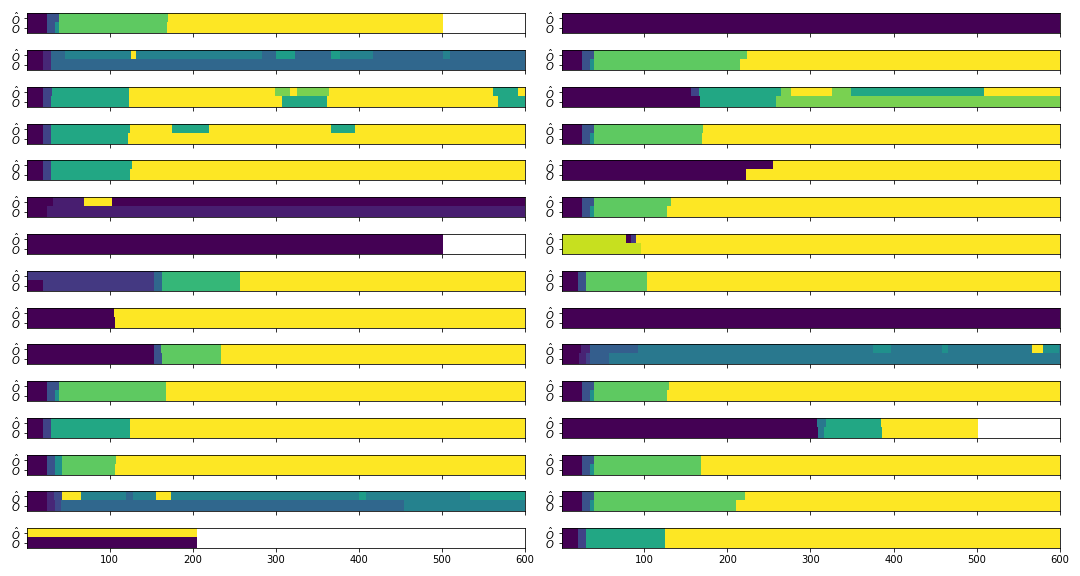
\includegraphics[width=\linewidth]{ASE_files/test_0.png}
    % \Description[States in time diagram]{A figure that color-codes the true and predicted states}
    \caption{Evaluation of the model on 30 random test data. Each graph shows the states in one run of the system. The colors show the states. The top-half of each plot depicts model's prediction of the system states ($\hat{O}$) and the bottom-half shows the true labels($O$). Since the output is one-hot encoded, the item with the most probability is used as the predicted label at each point in time. X-axis is the time axis. Only the first 600 samples (2 minute of simulation) are shown to improve legibility.}
    \label{fig:test_0}
\end{figure*}

\subsection{RQ3 Results: CPD Performance on Paparazzi (replication)}
\hl{NEW SECTION}
The results of applying baseline algorithms on Paparazzi data set can be seen in table~\ref{tab:cpd_paparazzi}.
The numbers are quite varied, there are scores worse then 1\% as well as some 100\% recall scores. The 100\% recalls are accompanied with a low precision; achieving that is not difficult. A method that outputs every point as a change-point will get similar results. The setting that got most of the best numbers is Pelt algorithm using an L1 cost function and a high penalty coefficient of 1000. However, please note that Pelt is a quite slow algorithm that could easily become infeasible to run on larger data set, as it was the case for MP's study. As a matter of fact, in this study getting the results for Pelt took more than 14 hours on the same machine that performed all other CPD algorithms in less than 1 hour. What you see in table~\ref{tab:cpd_paparazzi} is the summary of the results of more than 23800 experiments. 

Comparing the baseline results with the neural network model's results in the last three rows of the table, you can see improvements of 48.9\%, 26.83\%, and 11.46\% in F1 scores compared to the best numbers in the baselines (for $\tau = 1, 3, 5$ seconds respectively). Although this model still performed better than the baselines, the improvement margin was higher in the MP study (See the RQ1 results summary box and the paragraph above that in section~\ref{sec:results}). However, you can see that the scores that this approach achieved are not low, but the baselines could do a better job on Paparazzi's data compared to MicroPilot's, therefore shrinking the margin of improvement. It can be due to the fact that the new data set is tiny compared to MP, classic machine learning algorithms can do better so a deep learning model cannot shine here as it could for MP. To reiterate, Paparazzi data set consists of ~300 tests vs. ~900 tests in MP, and simulation lengths are up to 2500 samples vs. 18000 sample tests in MP's data set. It is worth mentioning that both in the original study on MP's data and here, the variation in baselines performances was way higher while my deep learning approach shows a more consistent performance; check the second column (recall with $\tau=1$s) for example. 

\begin{sidewaystable}
    \centering
\resizebox{\columnwidth}{!}{%
\begin{tabular}{llcccccccccc}
\toprule
  \textbf{Cost Function} &
  \textbf{Search Method} &
  \textbf{Penalty} &
  \textbf{Prec.} &
  \textbf{Recall} &
  \textbf{F1} &
  \textbf{Prec.} &
  \textbf{Recall} &
  \textbf{F1} &
  \textbf{Prec.} &
  \textbf{Recall} &
  \textbf{F1} \\
                                                  &              &   & \multicolumn{3}{c}{$\tau=1$s} & \multicolumn{3}{c}{$\tau=3$s} & \multicolumn{3}{c}{$\tau=5$s} \\  \toprule
\multirow{3}{*}{\textbf{Autoregressive Model}}
    & bottomup & 500  &       13.65\% &    14.13\% & 18.89\% &        39.73\% &     36.40\% & 36.14\% &        57.11\% &     53.20\% & 50.04\% \\
    & exact & 500  &       13.56\% &    13.85\% & 19.03\% &        39.67\% &     36.17\% & 36.03\% &        56.97\% &     52.89\% & 49.83\% \\
    & window & 100  &       15.97\% &     7.59\% & 13.54\% &        45.47\% &     20.40\% & 29.56\% &        64.16\% &     30.76\% & 41.20\% \\ \midrule
\multirow{3}{*}{\textbf{Least Absolute Deviation}}
    & window & 100  &       24.50\% &    15.92\% & 19.85\% &        56.39\% &     37.24\% & 44.53\% &        68.94\% &     48.20\% & 56.23\% \\
    & exact & 1000 &       \textbf{26.74\%} &    34.08\% & 29.92\% &        \textbf{60.77\%} &     77.32\% & \textbf{67.74\%} &        \textbf{74.73\%} &     93.16\% & \textbf{82.61\%} \\
    & bottomup & 1000 &       26.66\% &\textbf{34.99\%}& 30.35\% &        60.11\% &     78.14\% & 67.61\% &        72.85\% &     92.94\% & 81.30\% \\ \midrule
\multirow{3}{*}{\textbf{Least Squared Deviation}}
    & window & 1000 &       25.01\% &    16.14\% & 20.26\% &        54.58\% &     35.77\% & 42.96\% &        68.73\% &     48.11\% & 56.18\% \\
    & exact & 1000 &       21.28\% &    80.04\% & 33.49\% &        51.05\% &     99.58\% & 67.20\% &        65.36\% & \textbf{99.97\%} & 78.76\% \\
    & bottomup & 1000 &       21.30\% &    81.24\% & \textbf{33.62\%} &        50.98\% &\textbf{99.50\%}& 67.12\% &        65.24\% &\textbf{99.97\%}& 78.66\% \\ \midrule
\multirow{3}{*}{\textbf{Linear Model Change}}
    & bottomup & 100  &        7.39\% &     0.39\% &  9.98\% &        27.44\% &      1.49\% & 10.27\% &        52.51\% &      2.75\% &  9.90\% \\
    & window & 100  &        7.39\% &     0.39\% &  9.98\% &        27.44\% &      1.49\% & 10.27\% &        52.51\% &      2.75\% &  9.90\% \\
    & exact & 100  &        7.39\% &     0.39\% &  9.98\% &        27.44\% &      1.49\% & 10.27\% &        52.51\% &      2.75\% &  9.90\% \\ \midrule
\multirow{3}{*}{\textbf{Gaussian Process Change}}
    & window & 100  &        7.39\% &     0.39\% &  9.98\% &        27.44\% &      1.49\% & 10.27\% &        52.51\% &      2.75\% &  9.90\% \\
    & exact & 100  &        7.39\% &     0.39\% &  9.98\% &        27.44\% &      1.49\% & 10.27\% &        52.51\% &      2.75\% &  9.90\% \\
    & bottomup & 100  &       12.42\% &   \textbf{100.00\%} & 22.03\% &        33.15\% &    \textbf{100.00\%} & 49.55\% &        49.04\% &    \textbf{100.00\%} & 65.47\% \\ \midrule
\multirow{2}{*}{\textbf{Rank-based Cost Function}}
    & exact & 100  &       21.11\% &    31.85\% & 25.51\% &        52.29\% &     74.63\% & 61.13\% &        65.88\% &     89.30\% & 75.46\% \\
    & bottomup & 100  &       20.55\% &    31.84\% & 25.17\% &        49.97\% &     73.22\% & 59.04\% &        64.57\% &     89.35\% & 74.61\% \\ \midrule
\multirow{3}{*}{\textbf{Kernelized Mean Change}} 
    & bottomup & 100  &       15.66\% &     1.90\% &  9.45\% &        44.23\% &      5.36\% & 12.95\% &        62.37\% &      7.48\% & 15.66\% \\
    & exact & 100  &       14.07\% &     1.64\% &  9.77\% &        42.06\% &      4.74\% & 12.59\% &        60.92\% &      6.67\% & 14.56\% \\
    & window & 100  &        8.31\% &     0.61\% &  9.97\% &        29.38\% &      2.02\% & 10.60\% &        53.34\% &      3.39\% & 10.79\% \\ \midrule \midrule
\multirow{3}{*}{\textbf{My approach}} 
    & \multirow{3}{*}{\textbf{Data set:}}  
         & \textbf{Validation} &  45.63\% &    55.46\% & 50.07\% &   81.39\% &     90.97\% & 85.92\% &   88.38\% &     97.12\% & 92.54\%  \\
    & {} & b\textbf{Test (Tuning)} &  42.65\% &    54.87\% & 47.99\% &   76.73\% &     90.96\% & 83.24\% &   85.18\% &     97.46\% & 90.91\%  \\
    & {} & \textbf{Training}  &  39.81\% &    51.96\% & 45.08\% &   75.69\% &     90.62\% & 82.49\% &   84.96\% &     97.55\% & 90.82\%  \\
\bottomrule
\end{tabular}%
}
    \caption{Change point detection methods performance on Paparazzi data set. Since the 100\% recalls are actually outliers, the next largest recall values are in bold face as well.}
    \label{tab:cpd_paparazzi}
\end{sidewaystable}

\subsection{RQ4 Results: Multi-class Classification Performance on Paparazzi (replication)}
\hl{NEW SECTION}
In table~\ref{tab:rq2-1-results-replicate} the comparative results of the aforementioned algorithms with my method is presented. 
To compare with the original study, we can see that in all but two settings limiting the maximum number of features did not help improve the model. Another similar observation is that the scores do not vary very much with changing the window size, and decision trees almost universally outperform linear classifiers.
The scores themselves are just around the same values as well: Ridge classifier F1 score here is in 21-29\% which was 32-39\% in the original study, for decision trees it is in 67-68\% here and it was 73-77\% in the original study. 

The deep learning model's performance measures (on validation data) can be found in the last row of the table. 
You can see an $(81.92-68.96)-1=18.79\%$ improvement in F1 score, over the baselines. It confirms that this method can beat the best performing baselines in classifying input samples into the system's internal states. The improvement in the original study was 16.83\%. This, again confirms the reproducibility of the results from 

\begin{table}
\caption{Precision, recall, and F1 score of ridge classifiers (linear classifiers with L2 regularization) and decision tree classifiers with different sliding window widths ($w$). In this table, we only show the results of the best performing model in each group.}
\label{tab:rq2-1-results-replicate}
\resizebox{\linewidth}{!}{%
\begin{tabular}{llcccc}
\toprule
\textbf{w} &
  \multicolumn{1}{c}{\textbf{Classifier}} &
  \multicolumn{1}{c}{\textbf{Max Features}} &
  \multicolumn{1}{c}{\textbf{Precision}} &
  \multicolumn{1}{c}{\textbf{Recall}} &
  \multicolumn{1}{c}{\textbf{F1}} \\ \midrule
 3 &  Ridge &            - &      44.82\% &   14.45\% & 21.85\% \\
 3 & Decision Tree & $\sqrt{10w}$ &      61.88\% &   73.56\% & 67.22\% \\ \midrule
 5 &  Ridge &            - &      46.62\% &   15.10\% & 22.81\% \\
 5 & Decision Tree &            - &      64.28\% &   73.00\% & 68.36\% \\ \midrule
10 &  Ridge &            - &      47.59\% &   16.29\% & 24.27\% \\
10 & Decision Tree &            - &\textbf{65.06\%}& 73.36\% &\textbf{68.96\%}\\ \midrule
15 &  Ridge &            - &      44.41\% &   17.33\% & 24.93\% \\
15 & Decision Tree &            - &      63.53\% &   74.68\%& 68.65\% \\ \midrule
20 &  Ridge &            - &      57.97\% &   19.10\% & 28.74\% \\
20 & Decision Tree &            - &      64.72\% &   73.36\% & 68.77\% \\ \midrule
25 &  Ridge &            - &      62.13\% &   19.66\% & 29.87\% \\
25 & Decision Tree & $\sqrt{10w}$ &      61.17\% &\textbf{75.18}\% & 67.45\% \\ \midrule \midrule
   & \multicolumn{2}{l}{Proposed Method} & \textbf{71.13\%} & \textbf{88.69\%} & \textbf{81.92\%} \\
\bottomrule
\end{tabular}%
}
\end{table}

They say a picture is worth a thousand words\footnote{missing citation}, to better see the predictions of the deep learning model compared to the ground truth, see figure~\ref{fig:paparazzi_predictions}. 
\begin{figure}
    \centering
    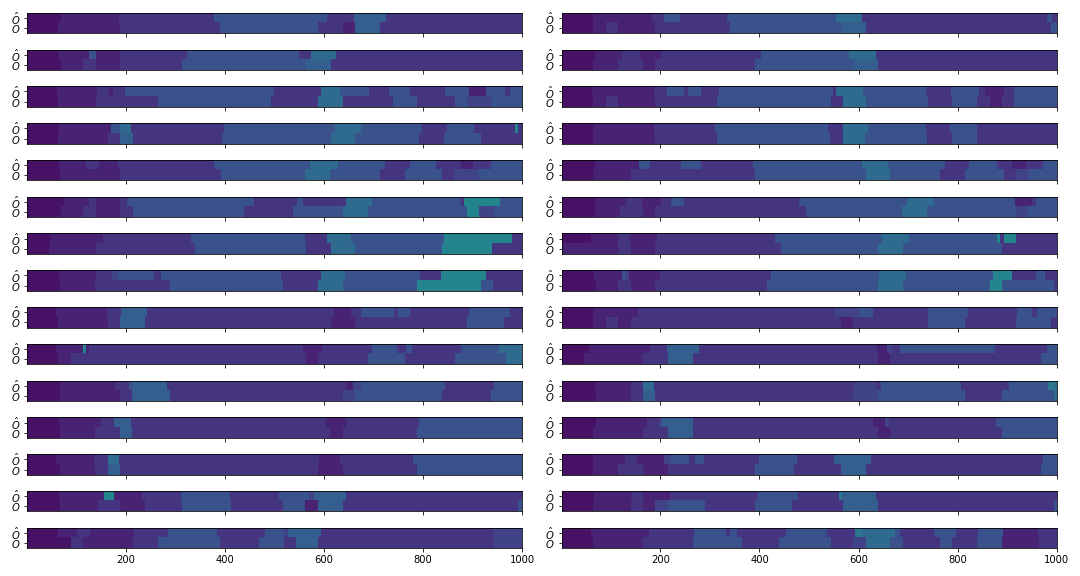
\includegraphics[width=\columnwidth]{6_files/states_chart.png}
    \caption{The states are color coded and each rectangle shows one test, only the first 1000 samples (200 seconds) are shown for more clarity. The same as figure~\ref{fig:test_0} in the previous chapter, the top half of each rectangle shows the model's output and the bottom half shows the true labels.}
    \label{fig:paparazzi_predictions}
\end{figure}

\subsection{RQ5 Results: Hyper-parameter Tuning}
\hl{NEW SECTION}
I used Tensor Board to visualize and compare the effects of different hyper-parameters on the model's performance. First, for a sanity check, I visualized 4 metrics, precision and recall in detecting change points with a small tolerance of $\tau=1s$, and precision and recall in estimating the internal state. A healthy linear and positive correlation is visible between all pairs of these metrics, it means that trying to improve one usually will not come at the expense of others. 
\begin{figure}
    \centering
    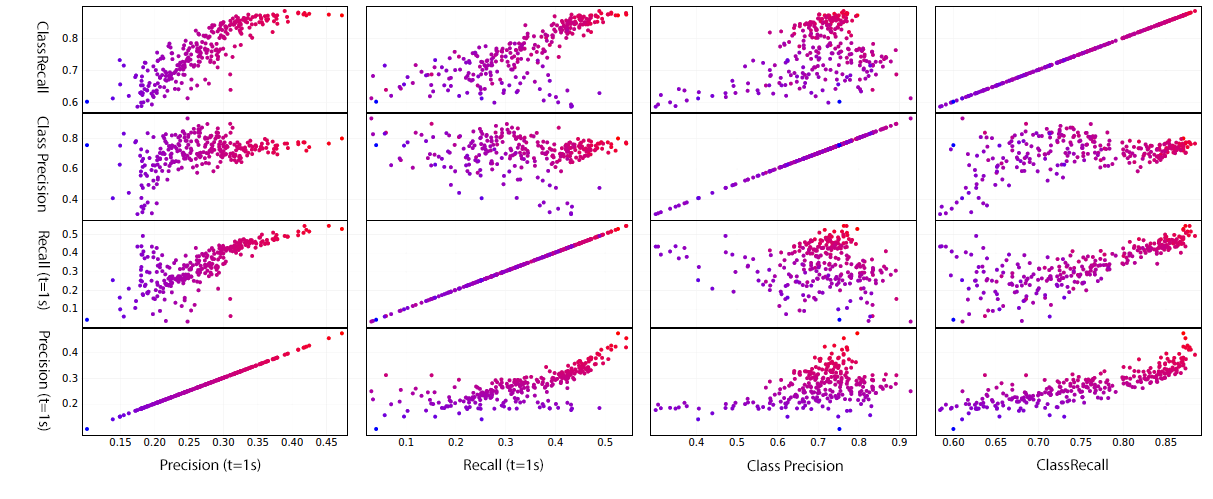
\includegraphics[width=\columnwidth]{6_files/prec_recall_matrix_tuning_white_background.png}
    \caption{Matrix of scatter plots comparing precision and recall of the deep learning model on test data.}
    \label{fig:precision_recall_matrix}
\end{figure}

Filtering the data to find the commonalities of better hyper-parameters shows that the number of GRU cells has a high correlation with both CPD precision and classification precision. 
It also shows that the kernel sizes and number of convolutional layers does not have an as strong correlation with higher precision and recalls. The number of convolutional filters in each layer has a bigger impact on the performance than the size of the kernels does. 
It makes sense because training larger kernels gets harder and harder and requires more data. Also, based on the previous studies, especially in the field of computer vision, we can say that each filter learns one feature so it is more effective to have many small filters that are easier to train and can learn multiple features of the data.
Therefore we can reduce the size of convolutional section of the model and use more recurrent cells to boost the performance without adding too many parameters. I performed another set of tests in a smaller search space to further optimize the hyper-parameters.

The new search space was all the combinations of these hyper-parameters:

\begin{enumerate}
    \item Learning rate, options being: $3\times10^{-4}$, $1\times10^{-3}$, and $3\times10^{-3}$
    \item Number of GRU cells, options: 128, 256, 384, and 512
    \item Number of convolutional filters in each layer: 32, 64, and 72
\end{enumerate}

\begin{figure}
    \centering
    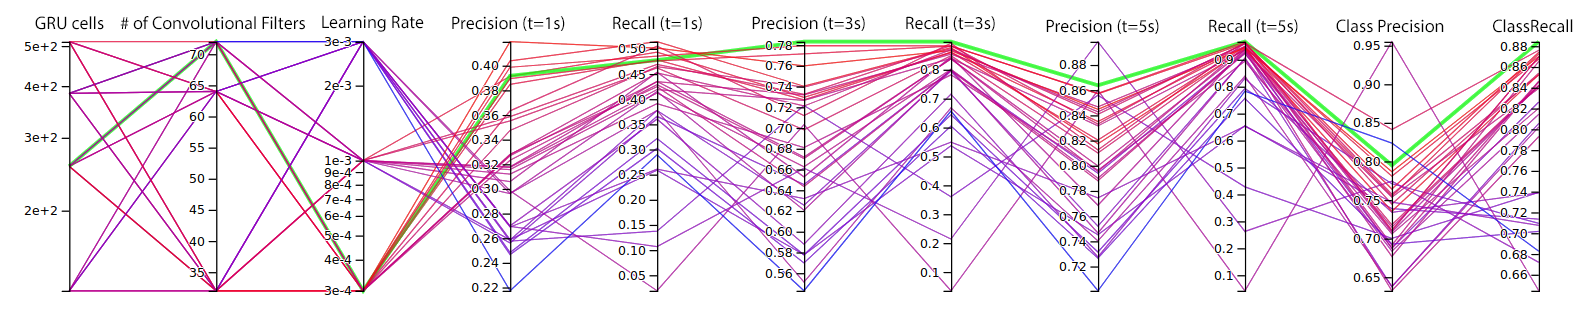
\includegraphics[width=\columnwidth]{6_files/refined_prec_recall_white_background.png}
    \caption{Parallel coordinates view showing the effects of select hyper-parameters on the performance measures.}
    \label{fig:precision_recall_parallel_coordinates}
\end{figure}
The results of the second round of tuning are shown in figure~\ref{fig:precision_recall_parallel_coordinates}. This chart shows 3 + 8 parallel axis, 3 hyper-parameters and 8 metrics. To make it more legible, the results with lower than 70\% precision ($\tau = 5s$) are omitted.
The green highlighted line is the best configuration tried, with the highest area under the curve. That configuration has the best or close to the best performance in all metrics. The configuration is to use 256 GRU cells, 72 filter per layer, and the lower learning rate of $3\times10^{-4}$.

I used these hyper-parameters to train the best model. The scores used in the research question 3 and 4 are the evaluation results of this model on the [previously unseen] validation data. The stopping criteria on training the model was for the validation loss to plateau, with a `patience' of 15 epochs. The optimizer converged in 54 epochs, after less than 3 minutes of training. 

The result of this tuning was a model with fewer convolutional layers and smaller kernel sizes but with more convolutional filters and recurrent layers that could perform better than the baselines. This shows having more and smaller convolutional filters is more effective in capturing local features in the data compared to having a small number of large filters (with kernels of size 20 for example which has 200 parameters). It also shows the important role that recurrent layers play in discovering long-term relations between inputs and outputs. 


\section{Limitations and Threats to Validity} \label{sec:threats_to_validity}
One of the limitations of our approach is that it might miss an input-output invariant correlation. It can happen when the input remains constant or it changes too little to reveal its relation with certain outputs. 
%In addition, as mentioned before, our approach relies on changes in signals. 
We assume that during the data collection, sampling happens in regular intervals; our approach probably will have a hard time achieving high performances, working on unevenly spaced time-series data.
%Maybe the CPD baselines could perform better if they were boosted by feature engineering, but the feature engineering task is can quickly become an arduous and inefficient. 
%It exists so it compensates for inability of traditional non-deep-learning methods in discovering meaningful features in the data. \cite{bengio2013deep}

In terms of construct validity, we are using standard metrics to evaluate the results. However, the use of tolerance margin should be taken with caution since it is a domain-dependant variable and can change the final results. To alleviate this threats, we have used multiple margins and reported all results. In terms of internal validity threats, we reduced the threat by not implementing the CPD baselines by ourselves and rather reusing existing libraries. In terms of conclusion validity threats, we have used many (888) real test cases from Micropilot's test repository and provided a proper train-validation-test split for training, tuning, and evaluation. \hl{Finally, in terms of external validity threats, our study suffers from being limited to only one case study. However, the study is a large-scale real-world study with many test cases. We plan to extend this work with more case studies from other domains, to increase its generalizability.}


 

\include{8_Conclusion}


% \chapter{Data Collection and Fuzzy Test Generation for Auto Pilots}\label{chapter:fuzz_tester}
\section{Introduction}
Model inference techniques are generally grouped into static and dynamic analysis categories. 
Static approaches use the code as their input data. They are able to gather all the required information such as function call graphs for example from the source code itself without a need to run the software.
A typical dynamic model inference pipeline, on the other hand, starts with running existing tests in the software to collect required data. \cite{Papadopoulos2015} 
The data that is generated in software run time is quite varied; It can range from the logs, to function calls, to network packets, to syscalls, and so forth. There are several aspects to be considered for this matter: what kind of data is needed, how are they going to be collected, what kind of model we are looking to have, and how are they going to be used in model inference. 

Walkinshaw et al. for example, \cite{walkinshaw2016inferring} sought to create state models as extended finite state machines. Their approach requires two collections of ordered events to work, a collection of positive examples which are events generated during a successful execution of the software as well as a set of negative examples. Each event there, is a function call; the log contains the list of functions that were called along with their parameters. 
In \cite{howar2012inferring} the events are high level actions such as `user registered` and `user logged in'. It also seeks to generate state models.
In Synoptic \cite{schneider2010synoptic} the communications in a distributed system is being modeled as an automata and the events are the logs generated by its components.


In this study the goal is to infer a state model of the system under study as a black-box without access to its source code. Therefore I am limited to observing the inputs and outputs of the system. Another piece of information that is often overlooked is time. In this study time is taken into consideration as well. I capture all the inputs and output values of the system in regular intervals. Since they are all numeric, they make a multivariate time series that I use to generate time-aware state models. 


A common theme in almost all model inference algorithms developed in the past two decades is that they use the data collected as the system functions in the wild. They either run existing test cases or instrument and inspect the system being used in production. 
This is to have a diverse collection of data that is also meaningful and representative of the actual system behaviour in common use cases.

Depending on the system under study and the type of data required, this might be an excellent way of collecting the data or might be infeasible for scalability reasons for example. That is what I encountered earlier while applying white-box model inference approaches to the industry partner's code base. The results are published in an ICPC 2019 paper \cite{mashhadi2019empirical}; to summarize that paper, the state of the art white box model inference algorithms suffer from not being scalable to be used in industry as is.
%In this study in particular there is an amalgam of both ends of the spectrum. 
As mentioned earlier, it is done on two auto pilot systems, Micro Pilot and Paparazzi. \cite{hattenberger2014using}
Although they both are highly capable and widely used drone auto pilots, their implementations are quite different which makes data collection phase quite different too.

\section{Data Collection Process}
In this section more details on how data was collected from each system will be presented. 

\subsection{MicroPilot AutoPilot}

Since a detailed overview of the data collection is discussed later in the next chapter, more specifically section~\ref{sec:mp_data_collection_process}, in this section I will only cover the related technical details about this process in MicroPilot. That is just to prevent restating what is already covered in the manuscript.

\subsubsection{Instrumentation}
Control decisions in this software are made in a 5Hz loop, it means that every 200ms all the sensor inputs are read and based on the current state of the aircraft and the system's goal at the moment (e.g. maintaining a constant speed) decisions will be made and output is generated. Considering this, the best way to capture those data is in the end of each iteration of this loop. I inserted instrumentation code there, to log input and output values at the exact spot where they are updated. 
Please note that although it is more convenient to capture the values in this way, it does not give us any special advantage or insight that breaks the black-box condition. In other words, the exact same data could be collected from the compiled binaries without any access to the internals, just with extra steps. Inputs and outputs, after all, are the very least thing available in both black-box and white-box settings.

\subsubsection{Test Scenarios}\label{sec:mp_test_scenarios}
MicroPilot has a repository of more than 900 system tests which can be run in a realistic simulator. The auto pilot can be used in SWIL and HWIL modes \cite{melmoth2019true}, which stand for software in the loop and hardware in the loop respectively. We used SWIL mode as it provides what we need without any of the overheads associated with HWIL mode. 

\subsection{Paparazzi}\label{sec:paparazzi_data_collection}

\subsubsection{Instrumentation}
Paparazzi provides a rich and flexible API that can be configured to record several different parameters in flight. The aircraft periodically sends data back to the ground station over a wireless link using a protocol called Paparazzi link. Paparazzi link is built over Ivy, a message bus protocol that uses UDP. 
In Paparazzi's architecture a process called `link' interfaces the wireless link to the aircraft to the computer's network; on one side are the Paparazzi link messages that come and go as UDP datagrams and on its other side is the (often wireless\footnote{A wired connection is used in HWIL test mode as well as some scenarios where the AutoPilot equipment is used in a autonomous submarine rather than an autonomous unmanned aircraft.}) connection to the aircraft.
In simulations, the modem and wireless communications are no longer needed, instead the auto pilot runs as a separate process and mimics a wireless channel over the local network. (See Figure~\ref{fig:paparazzi_comm_agents})

\begin{figure}
    \centering
    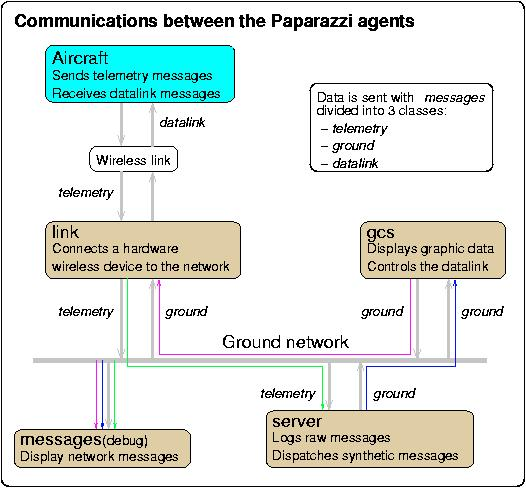
\includegraphics[width=\columnwidth]{4_files/Pprz_communication_agents.jpg}
    \caption{High level overview of communication links architecture in paparazzi \cite{hattenberger2014using}}
    \label{fig:paparazzi_comm_agents}
\end{figure}

Paparazzi comes with a multitude of small tools that could do most of what I needed in terms of instrumentation. There is a remote logger and a log player which are quite close to the instrumentation tool I need, however upon trying them in action, I figured that they cannot record some of the information that I need. Therefore, I developed a custom flight data recorder tool. 

\subsubsection{Test Scenarios}
Unlike MicroPilot that had a quite a number of system tests (in addition to other types of tests such as unit tests which I did not use), Paparazzi comes with only unit tests. As it is an open source software under GPL licence it comes with no warranty and also does not need certain certifications and approvals that commercial systems require, therefore incentives to have such tests are lower. 
Although it is a reliable and widely used auto pilot, it owes that reliability more to its widespread use in action (by many researchers and enthusiasts) rather than automated tests that verify its behaviour.
In this situation, where many eyes are watching over the code, bugs are discovered and patched quickly. However, to the best of my knowledge they are not recorded as system tests that verify the bugs are properly patched and detect regressions in the future.

To fill the void, I created a tool that can automatically generate valid and meaningful automated system tests for Paparazzi, run them automatically, and integrate with the flight data recorder tool to generate the data set for downstream tasks. It is called Pprz Tester and the source code, version history, project planning data (bugs, enhancements, tasks and issues, etc), and the documentations are available on GitHub at \url{https://github.com/MJafarMashhadi/pprz_tester}. 

In addition to that, I needed to patch some parts of Paparazzi to make the logging and testing more similar to MicroPilot, for example increase telemetry reporting rate from 2Hz to 5Hz. A list of these patches including the reason why that change was necessary or beneficial and the exact lines of code that need to be changed is available in the project wiki at \url{https://github.com/MJafarMashhadi/pprz_tester/wiki/Paparazzi-Patches}.

Aside from the patches, I found some bugs, missing features, missing documentations, and bad smells in the code that needed to be fixed. I contributed new code and documentation to the Paparazzi project to address these issues. The contributions were useful, up to the standards, and welcome in the project; they are included in the latest release\footnote{as of August 1st, 2020} of Paparazzi auto pilot: version 5.16.

\section{The Testing and Data Processing Tool Set}
I implemented the pipeline of generating tests, running them, and aggregating flight logs in an integrated tool with three components, one for each stage. In the following sections I will explain these components and their role in the system. I also explain how event-driven programming paradigm was implemented here both to decrease coupling and to make it more resilient to unexpected or buggy behaviour. It is necessary for two reasons: 1. as a testing tool, it is \textit{expected} to encounter bugs in software under test and should be resilient to them 2. the message passing design of Paparazzi architecture, in addition to its ability to support multiple aircraft in flight at the same time left me with no choice but to use an event-driven design.


\subsection{Flight Data Recorder}
Although paparazzi comes with a logging feature in its `server' component (Figure~\ref{fig:paparazzi_comm_agents}), it only logs a subset of required data. Furthermore, the data comes in separate messages with different frequencies; for example speed updates are sent in \verb|AIRSPEED| message once a second, orientation updates and engine rpm are reported in \verb|ATTITUDE| and \verb|ENGINE_STATUS| messages respectively which are dispatched every 200 milliseconds, while servo outputs are only sent once every 5 seconds. All these data need to be aggregated and aligned. Please refer to the Table~\ref{tab:pprz_messages} in \hyperref[appendixa]{Appendix~A} for a full list of messages used.

The most flexible option with the least overhead is to have an independent module that understands Paparazzi link, captures these messages and does data aggregation and logging in real-time. So I created a flight data recorder to collect all the required data from telemetry messages.

In the beginning the instance of ``AircraftManager'' singleton class starts with listening for \verb|NEW_AIRCRAFT| messages. This message type notifies this class when new aircraft come online in the simulation. Then it sends a \verb|AIRCRAFTS_REQ| request message to server to get a list of currently online aircraft. The response to both of these messages are processed in the same way: The aircraft unique ID will be checked against the hash table of known aircraft, if it is a new one an ``Aircraft'' instance will be created and added to the hash table. (See the class diagram in Figure~\ref{fig:fdr_class_diagram} in \hyperref[appendixa]{Appendix~A})

Each ``Aircraft'' object in the makes a number of requests back and forth with other components in the system (server, data link, and the auto pilot process) to gather required information about that aircraft, including its flight plan. This class along with ``Aircraft Parameters'' and ``Aircraft Commands'' provide a unified programmatic API for monitoring and controlling the aircraft. 

I implemented observer pattern \cite{gamma1995design} in ``Aircraft Parameters'' to enable other components (such as flight data recorder and automated test executor) to listen for changes in the aircraft state and respond accordingly in an event-driven manner. 
After creation of an ``Aircraft'' object, as a part of its initialization, several observers are created and attached to it. A ``Record Flight'' instance is one of them. It observes new \verb|FLIGHT_PARAM| messages as well as changes in `throttle', `flight time', and `commands.values' parameters. This class stores and aligns these parameters in a pandas data frame which is stored on disk periodically. The data can be stored in a human-readable CSV file or as a compressed HD5 binary. Some data normalization and unit conversions (such as meters to feet) also happen before saving in order to make the generated data similar to MicroPilot's.

Supplementary UML diagrams are provided in \hyperref[appendixa]{Appendix~A}.


\subsection{Automated Test Executor}
The test executor takes the control of the aircraft by running prefabricated test scenarios. While the low leve control of the aircraft is done by the auto-pilot software (the system under test), it needs high level commands such as `climb to 200ft'. Automated test executor does that, using hand crafted test scenarios or the ones generated by the test generator component.

Tests scenarios are defined as subclasses of \verb|PlanBase| class. Each plan needs to override a method that returns an iterable of plan items which should be executed one by one. 
\begin{lstlisting}[language=Python, basicstyle=\linespread{0.1}]
class ExamplePlan(PlanBase):
  def get_items(self, **kwargs):
    block_name = kwargs.pop('block_name')
    circles = int(kwargs.pop('circles'))
    return [items.JumpToBlock(block_name),
      items.WaitForCircles(n_circles=circles)]
\end{lstlisting}
The above plan for example, takes a block name and a number of circles as its parameter and executes the two items in succession. An example of running this plan can be like the command below:
\begin{lstlisting}[language=bash]
$ run_test.py ExampleAircraft ExamplePlan\ 
    -Dblock_name='loiter' -Dcircles=2
\end{lstlisting}
Using this parameters is analogous to test parameterization in mature unit testing frameworks (such as pytest). It allows similar test plans that are only different in some parameters to be consolidated in one test case.
Using parameters also improves the reproducibility of test scenarios while improving its flexibility. Test scenarios (plans) do not need to include commands for waiting for aircraft to take off and land, the testing tool automatically wraps it with appropriate initialization code.

The core test plan runner is implemented as an observer class that listens for multiple messages and parameters to get notified about changes in the aircraft's state (See Figure~\ref{fig:flight_plan_executor_class_diagram} in \hyperref[appendixa]{Appendix~A}). It iterates over the flight plan items and calls their \verb|match| method to decide whether that item should be executed. Whenever a match is found the item will be executed and the iterator will move to the next test plan item. Consult Figure~\ref{fig:flight_plan_items_class_diagram} in \hyperref[appendixa]{Appendix~A} for a class diagram of all flight plan items.

Test plans should be importable from \verb|pprz_tester.generated_plans| module. The structure is simple and clearly defined so that they can easily be handcrafted (like the example above) or generated using the test generator component.

The test runner is tailored specifically for paparazzi in several ways:
\begin{enumerate}
    \item % First, 
As mentioned before, it takes care of aircraft initialization, take off, and landing
    \item %Second, 
It uses standard paparazzi environment variables such as \verb|$PAPARAZZI_HOME|.\footnote{If it is not set, the user can use \verb|-p /path/to/paprazzi| command line argument to set this value, and if that is not set too, a default value will be used.} 
    \item %Third, 
It can build the auto pilot if \verb|--build| argument is set so the user does not have to build it manually in Paprazzi center. 

    \item %Fourth, 
If \verb|--gcs| argument is set, the ground control station window will be opened (See Figure~\ref{fig:paparazzi_gcs}). It provides a real-time map that visualizes the aircraft path, waypoint locations, wind direction and velocity, and several other parameters of the aircraft such as their airspeed and altitude. 
    \item %And last, 
\verb|--no-sim| argument tells tester to not launch the simulator. Its use case can be when a physical auto pilot is being used (similar to MicroPilot's HWIL mode), or when for any reason the user chooses to run the simulator manually. 
\end{enumerate}

\begin{figure}
    \centering
    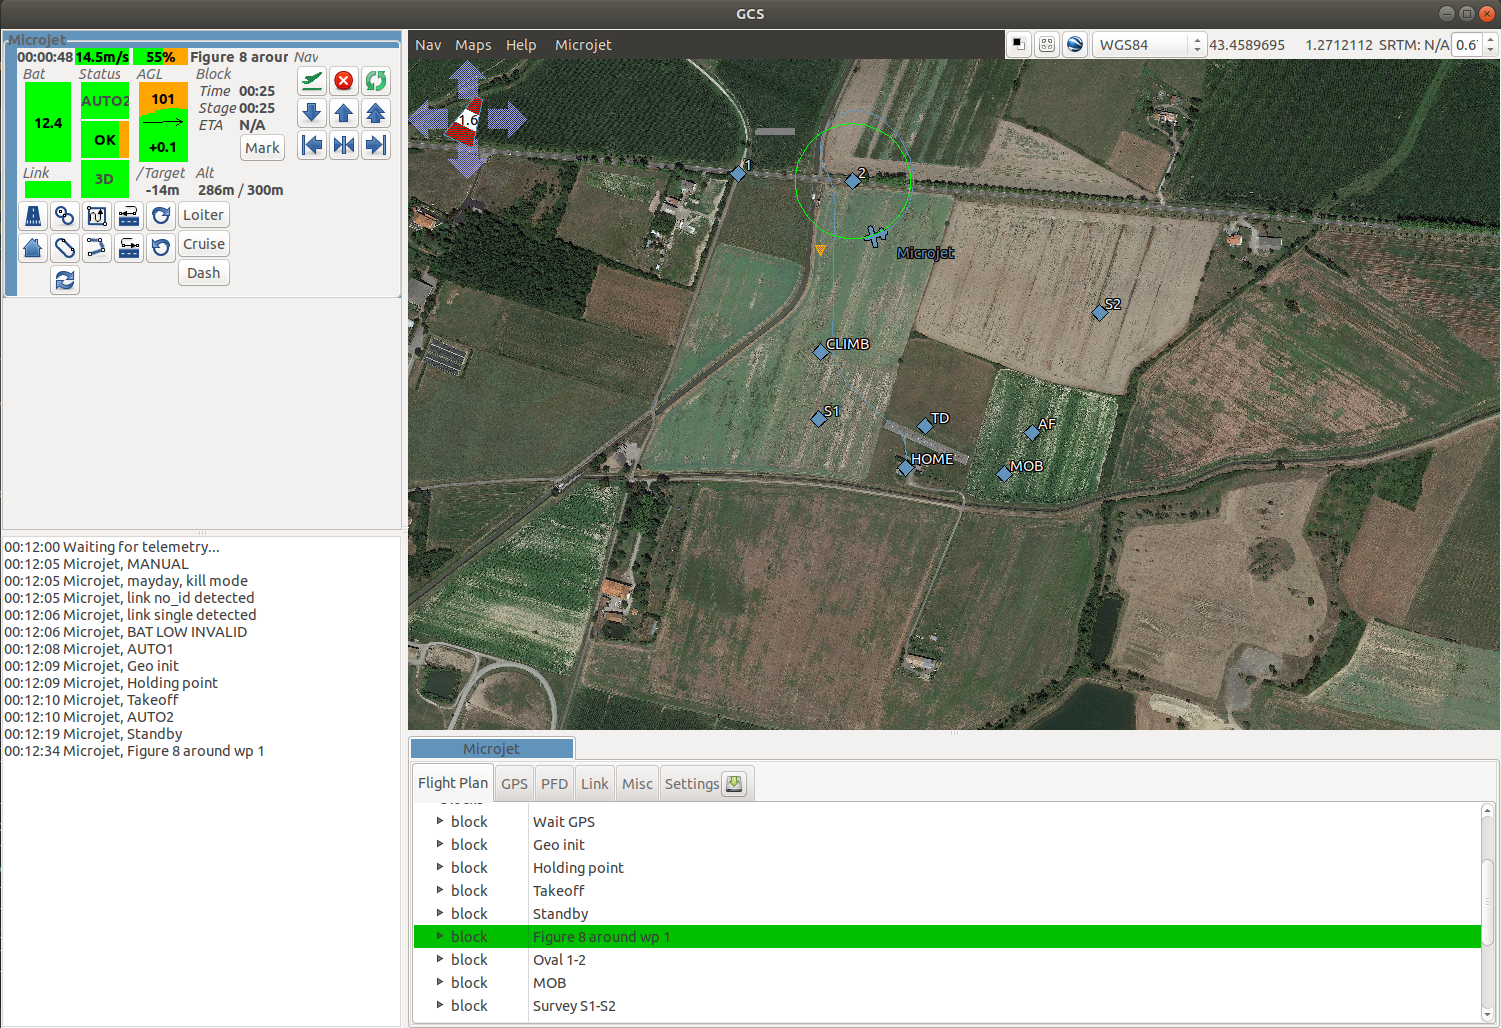
\includegraphics[width=\textwidth]{4_files/GCS.png}
    \caption{A snapshot of ground control station software (GCS), visualizing the map, waypoints (blue diamonds), the aircraft, its flight history (blue), the intended flight path (green), as well as its state (bottom in green) and some telemetry data (top left). The plan that it is following is one of the automatically generated test scenarios.}
    \label{fig:paparazzi_gcs}
\end{figure}

Test runner can move waypoints as well. The user can fix any number of waypoints at specified locations, providing their latitude longitude and altitudes. It can also randomize their location inside a cube. Boundaries of that cube (i.e. east-west, north-south, and floor-ceiling) are customizable through provided command line arguments.

The comprehensive list of command line arguments is included in Table~\ref{tab:test_runner_commandline_args} in \hyperref[appendixa]{Appendix~A}.


\subsection{Automated Test Generator}
The test generator component is a fuzz test generator specifically designed for Paparazzi. An auto pilot has plenty of parameters to change. Many of them need to remain unchanged. For example, changing aerodynamic and physical parameters of an air frame will make it behave incorrectly or even crash. A naïve algorithm might be tempted to only change these parameters to optimize a metric of ``bug''s per test. To comply with the constraints in input format and range and optimize test scenario diversity without having to have thousands of tests, I opted for developing a specialized automated test generator. 

This test generator is completely compatible with Paparazzi and designed with specific needs of an auto pilot in mind. It begins with loading and parsing the one fixed wing flight plan that comes with Paparazzi. It defines multiple actions (control blocks) available to a fixed wing aircraft. Two important components in the flight plan that are used are the waypoint names and locations, and available blocks. A test scenario is generated by taking the initial flight plan and fuzzing three parameters about it:
\begin{enumerate}
    \item Waypoint locations
    \item Sequence of actions 
    \item Action timing
\end{enumerate}

The test generator can be configured to fuzz all or some of them. I generated 31 tests with fuzzing the last two. Please note that the sequence of actions can have any length between 1 and the number of possible actions (5, in my case). Also for each sequence, $n!$ different permutations can be made that will result in very different outcomes. That makes the number of tests, $5!\times1+4!\times5+3!\times10+2!\times10+1!\times5=325$. Also note that these generated tests are made of unique blocks, in other words, a test scenario does not contain plans like ``Do A then B then A again'' while these plans are perfectly valid. In case one wants to have such plans they can write test plans manually.

The output is a python module that contains a subclass of \verb|PlanBase|, as expected by the automated test executor. These two work together seamlessly and the user can just use them in a plug-and-play manner without touching the code. Though, the generated code is designed to be effortlessly understandable and easily editable it even incorporates some auto-generated comments in the code.

The full table of command line arguments that test generator accepts is presented in Table~\ref{tab:test_generator_commandline_args} in \hyperref[appendixa]{Appendix~A}. To provide an example, the following command generates tests of length (number of actions) 2 for `Microjet' aircraft and writes it to the file \verb|l2.py| in the specified directory. It fuzzes the location (latitude, longitude, and altitude) of waypoint `S2' in the default cube, just overriding the altitude bounds in 200 to 220 meters, while the coordinates of `S1' are fixed. The initialization and landing stages which must be excluded from the test scenario are also specified. 
\begin{lstlisting}[language=bash]
gen_test.py --exclude "Wait GPS" "Geo init" "Holding 
point" Takeoff Standby "Land Right AF-TD" "Land Left 
AF-TD" land final flare --fuzz-wps S2 \
--wp-fuzz-bounds-alt 200 220 -w S1 43.4659053 1.27 300 \
--length 2 Microjet pprz_tester/generated_plans/l2.py
\end{lstlisting}
Some of the available actions and all the waypoints in this flight plan can be seen in Figure~\ref{fig:paparazzi_gcs}.

% \chapter{Replication and Extension}

\section{Introduction}

In the previous chapter, we have seen the results of applying my proposed model inference technique on the data collected from our industry partner, MicroPilot. However, to confirm the results and idea furthermore a second study on a similar software is quite helpful. In the second case study in addition to confirming that the technique is applicable on other software, I could improve on some aspects of the previous manuscript.

% TODO: a summary of the results

\section{The Case Study Subject}
I chose paparazzi auto pilot as an open-source alternative to MicroPilot's auto-pilot for replication. Paparazzi \cite{hattenberger2014using} project started in 2003 as an academic auto-pilot and continues to be developed with the state of the art in the autonomous flying vehicle's field. Another major player in open source auto-pilot software scene is ArduPlane. A comparison about how paparazzi is superior to ArduPlane can be read at \url{https://wiki.paparazziuav.org/wiki/Paparazzi_vs_X}. 
In addition to that, after doing a preliminary study, I found out that paparazzi has a more straightforward and robust protocol for remote controlling and data collection, as explained previously in section~\ref{sec:paparazzi_data_collection}. 
Furthermore, paparazzi supports multiple flight dynamic model (FDM) simulators. One of them is JBSim\footnote{\url{http://jsbsim.sourceforge.net/}} which provides an advanced physical model of complex dynamics in air-frames and sensors for an accurate and close to the reality simulation. 


\section{Objectives}
\subsection{RQ 1) Can the results be replicated with regards to state change point detection (CPD)?}
I ran 42 different combinations of settings for CPD algorithms in ``ruptures'' library \cite{Truong2018ChangePointSurvey}. 
There are 7 cost functions, 3 search methods (1 exact and 2 approximate), and 3 penalty values (100, 500, and 1000).
I used the same configurations in the previous study. 
To evaluate them, I used the same precision, recall, and F1 score (with a margin of tolerance) as the previous study which are defined in section~\ref{sec:CPD_metrics}.

\subsection{RQ 2) Can the results be replicated with regards to state detection?}
I fed the data to a number of classic machine learning algorithms as baselines. The problem setting is a multi-class classification, though with paparazzi the number of classes are smaller. 
There are 20 possibe states in Paparazzi as opposed to MicroPilot's 25. This is due to their differences in solving the problem of defining a mission and controlling an automated vehicle (the aircraft) to perform it.

\subsection{RQ 3) How will hyper-parameter tuning affect the results?}
In previous study the hyper-parameters of the neural network model were tuned manually. Hyper-parameters include the number of convolutional layers, number of convolutional filters in each layer, number of recurrent cells, and optimizer parameters such as learning rate. There are no gold standards for the values of these parameters, they need to be tuned for each problem. In the replication I opted for existing automated ways for finding better hyper-parameters.


\section{Experiment}
\subsection{Data Collection}
The process of collecting the data has already been explained in chapter~\ref{chapter:fuzz_tester} in detail. However, let us have a quick recapitulation:
Unlike MicroPilot, Paparazzi did not include any system tests. So, I developed a fuzz tester tool to generate valid, diverse, and meaningful test plans based on the example flight plan that is shipped with the software. My tool can automatically generate system tests, run them in a simulator (or on hardware\footnote{Although I have not tested running tests on a hardware (HWIL) to confirm, but having implemented the protocol it potentially is capable of doing so}), and also collect required telemetry data from the aircraft. The targeted randomizations in test inputs are augmented with the stochastic wind model in the simulation to further diversify the observed behaviours. My fuzz tester tool ran ran each generated scenario in a simulation and recorded the required flight data.
The result was 378 runs worth of different flight scenarios.
After collecting the data I performed some pre-processing steps on them to make them more similar to what the previous model was trained on. These pre-processing steps include normalizing some values as well as metric to imperial unit conversions.


\subsection{CPD baselines (RQ 1)}
Similar to the MicroPilot study, I fed the data from Paparazzi to several CPD baselines implemented in ``ruptures'' library.
Fortunately, with smaller data set size (in comparison to MicroPilot's), it was feasible (though still time-consuming) to try ``Pelt'' CPD method \cite{killick2012optimal} as well, making the replication study is richer in that sense. Pelt is the most efficient exact CPD method which, as mentioned before, failed to scale up to process MicroPilot's data. All other CPD methods are approximate algorithms.

\subsection{Classification algorithms (RQ 2)}
I used a ridge classifier and a decision tree classifier with 3 settings for maximum number of features with no limit on their depths. This setting is the same as the MicroPilot's case, with the only difference being having no depth limit. So, I ran overall $3\times6=24$ different settings for classic learning algorithms. 

\subsection{Hyper-parameter Tuning (RQ 3)}


\section{Results}
\subsection{CPD baselines (RQ 1)}


\subsection{Classification algorithms (RQ 2)}
In table~\ref{tab:rq2-1-results-replicate} the comparative results of the aforementioned algorithms with my method is presented. 
To compare with the original study, we can see that in all but two settings limiting the maximum number of features did not help improve the model. Another similar observation is that the scores do not vary very much with changing the window size, and decision trees almost universally outperform linear classifiers.
The scores themselves are just around the same values as well: Ridge classifier F1 score here is in 21-29\% which was 32-39\% in the original study, for decision trees it is in 67-68\% here and it was 73-77\% in the original study. 

% TODO: add my results too

\begin{table}
\caption{Precision, recall, and F1 score of ridge classifiers (linear classifiers with L2 regularization) and decision tree classifiers with different sliding window widths ($w$). In this table, we only show the results of the best performing model in each group.}
\label{tab:rq2-1-results-replicate}
\resizebox{\linewidth}{!}{%
\begin{tabular}{llcccc}
\toprule
\textbf{w} &
  \multicolumn{1}{c}{\textbf{Classifier}} &
  \multicolumn{1}{c}{\textbf{Max Features}} &
  \multicolumn{1}{c}{\textbf{Precision}} &
  \multicolumn{1}{c}{\textbf{Recall}} &
  \multicolumn{1}{c}{\textbf{F1}} \\ \midrule
 3 &  Ridge &            - &      44.82\% &   14.45\% & 21.85\% \\
 3 & Decision Tree & $\sqrt{10w}$ &      61.88\% &   73.56\% & 67.22\% \\ \midrule
 5 &  Ridge &            - &      46.62\% &   15.10\% & 22.81\% \\
 5 & Decision Tree &            - &      64.28\% &   73.00\% & 68.36\% \\ \midrule
10 &  Ridge &            - &      47.59\% &   16.29\% & 24.27\% \\
10 & Decision Tree &            - &\textbf{65.06\%}& 73.36\% &\textbf{68.96\%}\\ \midrule
15 &  Ridge &            - &      44.41\% &   17.33\% & 24.93\% \\
15 & Decision Tree &            - &      63.53\% &   74.68\%& 68.65\% \\ \midrule
20 &  Ridge &            - &      57.97\% &   19.10\% & 28.74\% \\
20 & Decision Tree &            - &      64.72\% &   73.36\% & 68.77\% \\ \midrule
25 &  Ridge &            - &      62.13\% &   19.66\% & 29.87\% \\
25 & Decision Tree & $\sqrt{10w}$ &      61.17\% &\textbf{75.18}\% & 67.45\% \\ \midrule
   & \multicolumn{2}{l}{Proposed Method} & \textbf{xx.xx\%} & \textbf{xx.xx\%} & \textbf{xx.xx\%} \\
\bottomrule
\end{tabular}%
}
\end{table}
\subsection{Hyper-parameter Tuning (RQ 3)}


\chapter{Conclusion} %  and Future Work?
I first experimented with white-box model inference of MicroPilot's source code using existing state of the art tools. 
However, the algorithms' implementations showed quite a number of scalability issues when tested with such a large scale software system. I was able to mitigate or even solve some of the issues through various methods and tricks, but still they were not usable as a robust model inference technique. These attempts were published in ICPC '19 (co-located with ICSE) in negative results track. \footnote{I referenced that paper \cite{mashhadi2019empirical} in this thesis but did not include it.}

Thereafter, considering the partner company's needs, I took a higher level black-box approach in modeling the software. Inspired by deep neural network architectures that showed good performance other fields (such as speech recognition, sleep phase detection, and human activity recognition) I came up with a deep neural network that combined convolutions and recurrent cells. Training this model using an appropriate loss function yielded promising results in inferring a behavioural model from the auto pilot execution data.

The results could be made stronger if they could be replicated on another similar software as well. Therefore I started working on applying the same method on an open source auto pilot software. Considering several aspects, I chose Paparazzi UAV auto pilot as the subject for the replication study. I created a tool that automatically generated fuzz test scenarios for fixed wing aircraft that use Paparazzi. It could also execute the tests and collect telemetry data for training the model down the way. 
I managed to replicate the study and get results as good as (in some cases even better) the first study on MicroPilot. In addition, I created a hyper-parameter tuning pipeline that significantly improved the results on Paparazzi's data; the default hyper-parameter values were [manually] tuned for MicroPilot.

To sum up: I developed a novel method for inferring black box models for auto pilot software systems, evaluated it on a large company's source code as well as a widely used open source solution. Along the way, I published two conference paper and one journal paper (which was also presented in ASE '19's journal-first-conference-second track), salvaged an old Java instrumentation tool (\url{https://github.com/sea-lab/JInstrumenter}) that is used for white-box analysis, and developed a fuzz test generator/executor/flight data recorder tool specialized for Paparazzi (\url{https://github.com/MJafarMashhadi/pprz_tester}). Also, I contributed ~10 pull requests to Paparazzi fixing bugs, adding features, etc which are included in its latest version during developing that tool.


% The back matter includes commands to produce endnotes, index,
% glossary, bibiliography, and the like.

\backmatter
% \printpagenotes
\bibliography{thesis}

% The appendix contains material that would clutter up the main text,
% such as program code, survey instruments, or interview transcripts.
% Remove it if you don't have an appendix.

\appendices
% \setcounter{figure}{0}
% \renewcommand\thefigure{\Alph{chapter}.\arabic{figure}}

% Sample University of Calgary Thesis
% This file contains the APPENDIX

% If there is just one appendix, it must be called ``Appendix.'' For
% multiple appendices, use \chapter and a descriptive title,
% e.g., \chapter{Questionnaires}

\chapter{Appendix~A: PprzTester documentations}\label{appendixa}

UML Diagrams and tables for the developed tools: flight data recorder, automated test generator, and automated test executor.
\begin{table}
    \centering
\begin{longtable}{llp{.50\columnwidth}}
\toprule
\textbf{Message Name }   & \textbf{Sent By }    & \textbf{Use}                                                                     \\ \hline
\endhead
%
\hline
\endfoot
%
\endlastfoot
%
PPRZ\_MODE &
  Aircraft &
  PprzTester listens to this message to find out when the auto-pilot software is booted up and is ready for flight. It also contains the state of active PID loops that is used to determine the internal state of the auto-pilot. \\
NAVIGATION &
  Aircraft &
  Contains the current active flight plan block as well as number of full circles the aircraft has completed among other data \\
COMMANDS        & Aircraft    & Contains commands from the auto-pilot to the servos (the outputs)       \\
FLIGHT\_PARAMS  & Aircraft    & Contains most of the sensor readings and required aircraft parameters   \\
ENGINE\_STATUS  & Aircraft    & Contains engine RPM and throttle among other parameters                 \\
CIRCLE\_STATUS &
  Aircraft &
  Contains detailed information about aircraft status while it is in circling mode. Overlaps with NAVIGATION to some extent \\
WAYPOINT\_MOVED & Server      & Sent in case any waypoints are relocated                                \\
MOVE\_WAYPOINT  & PprzTester & To update waypoint locations                                            \\
NEW\_AIRCRAFT &
  Server &
  Event of a new aircraft coming online in the network. It does not necessarily mean that it is ready for flight, should listen for PPRZ\_MODE as well \\
AIRCRAFTS\_REQ  & PprzTester & Request to get the list of active aircraft                              \\
AIRCRAFTS       & Server      & Response to the above request                                           \\
CONFIG\_REQ     & PprzTester & Request for an aircraft's configs                                       \\
CONFIG &
  Server &
  Response to the above request containing  its name, flight plan, DL settings, air frame parameters, etc. \\
DL\_SETTING     & PprzTester & Update a DL setting value. It is used to launch the aircraft in the air \\
JUMP\_TO\_BLOCK & PprzTester & Commands the aircraft to change active block to another block defined in the flight plan  \\ \bottomrule
\end{longtable}
\caption{Subset of all available messages in Paparazzi that are used in PprzTester tool}
\label{tab:pprz_messages}
\end{table}

\begin{table}
    \centering
\begin{longtable}{lp{.63\columnwidth}}
\toprule
\textbf{Argument}   & \textbf{Description}\\ \hline
\endhead
%
\hline
\endfoot
%
\endlastfoot
airframe              &  The aircraft to simulate \\
plan                  &  Plan name to run as a python module in \verb|pprz_tester.generated_plans| \\
--agent-name          &  Specify unique agent name on ivy bus \\
-l, --log             &  Log file directory \\
--log-format          &  The format to store and compress logs in, can be hd5 or csv \\ \hline
-p, --paparazzi-home  &  Directory in which Paparazzi source code is cloned in \\
-b,--build            &  Build the aircraft before launching the simulation \\
--gcs                 &  Open GCS window \\
--no-sim              &  Does not launch the simulator \\
--prep-mode           &  The required conditions before starting the flight scenario. It can be waiting for altitude to stabilize (climb) or waiting for a complete circle around stand by waypoint (circle) or both. \\ \hline
--fuzz-wps            &  Waypoints to fuzz locations of. Use * to fuzz all \\
--wp-fuzz-bounds-lat  &  Minimum and maximum latitude (south-north) to fuzz waypoint locations in \\
--wp-fuzz-bounds-lon  &  Minimum and maximum longitude (east-west) to fuzz waypoint locations in \\
--wp-fuzz-bounds-alt  &  The boundaries inside which waypoint altitudes are fuzzed \\
-w,--wp-location      &  Fix one or more waypoints' locations (overrides fuzzing) \\ \hline
-Dname=value          &  Optional plan arguments. They will be passed to \verb|get_items| as keyword arguments. \\ \bottomrule
\end{longtable}
\caption{Test runner command line arguments}
\label{tab:test_runner_commandline_args}
\end{table}


\begin{table}
    \centering
\begin{longtable}{lp{.63\columnwidth}}
\toprule
\textbf{Argument}   & \textbf{Description}\\ \hline
\endhead
%
\hline
\endfoot
%
\endlastfoot
airframe              &  The aircraft to generate tests for \\
output                &  Output file name or the directory to output the generated plans \\
-i, --include         &  Flight plan blocks to include in the generated plans \\
-x, --exclude         &  Flight plan blocks to exclude from the generated plans \\ 
-l, --length          &  Number of flight plan blocks to include. \\ \hline
-p, --paparazzi-home  &  \multirow{6}{*}{Shared with test runner in Table~\ref{tab:test_runner_commandline_args}}\\
--fuzz-wps            &   \\
--wp-fuzz-bounds-lat  &   \\
--wp-fuzz-bounds-lon  &   \\
--wp-fuzz-bounds-alt  &   \\
-w,--wp-location      &   \\ \bottomrule
\end{longtable}
\caption{Test runner command line arguments}
\label{tab:test_generator_commandline_args}
\end{table}


\begin{landscape}
\begin{figure}
    \centering
    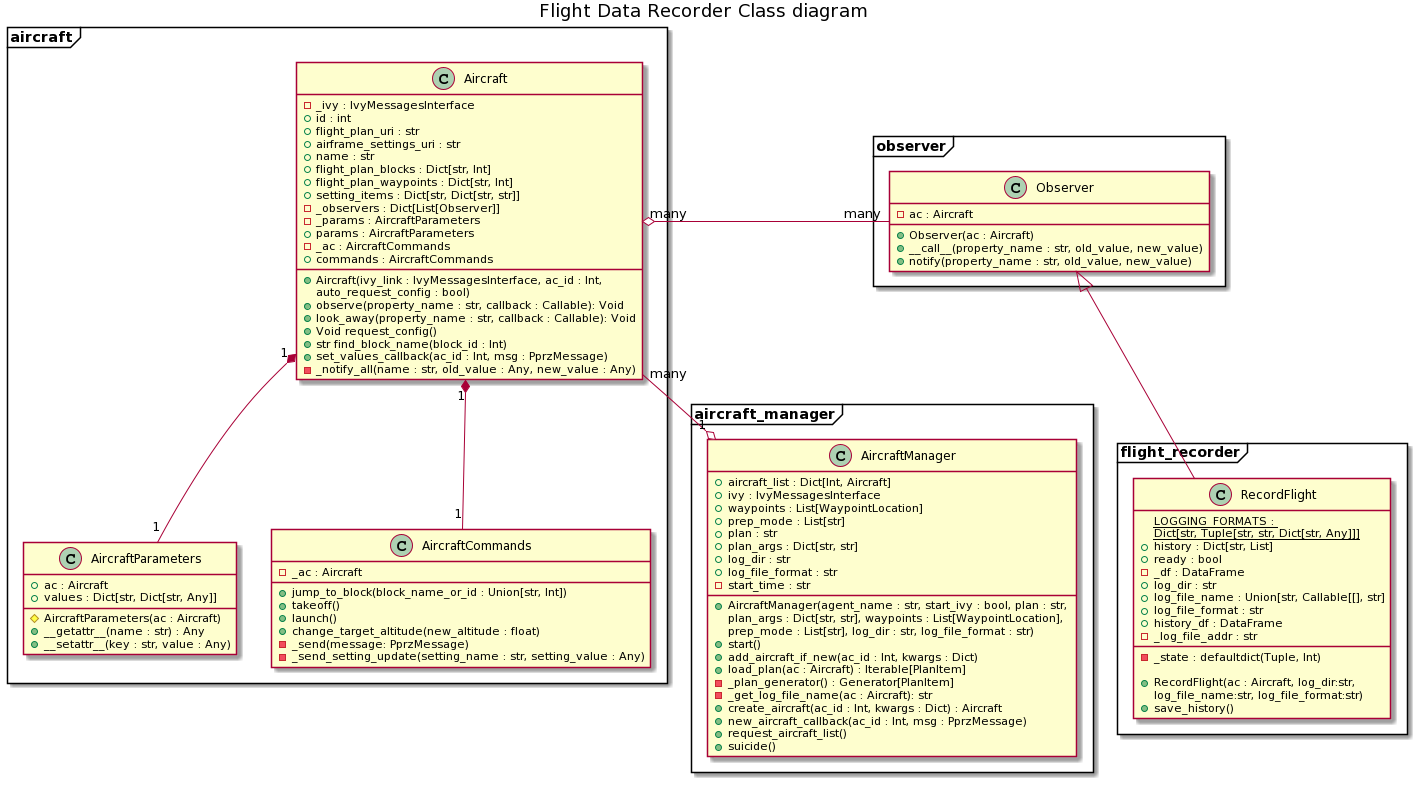
\includegraphics[width=\columnwidth]{UML/fdr_class_diagram.png}
    \caption{Class diagram for flight data recorder}
    \label{fig:fdr_class_diagram}
\end{figure}
\end{landscape}

\begin{figure}
    \centering
    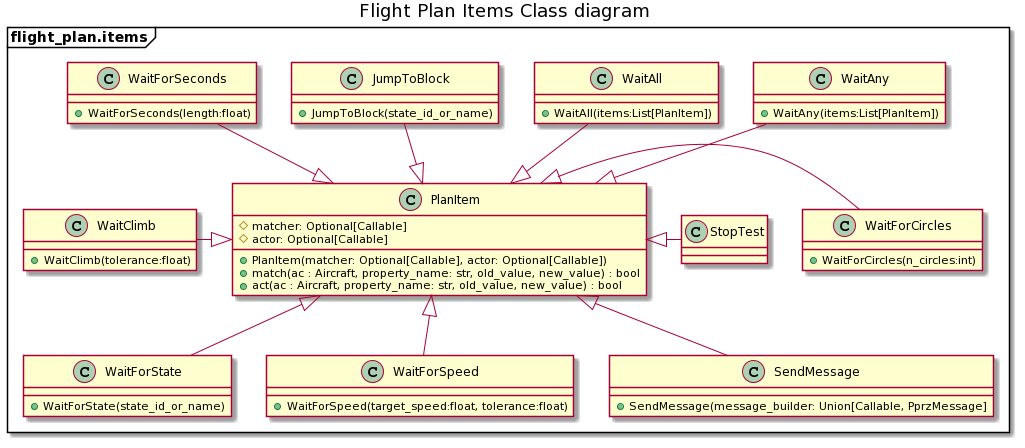
\includegraphics[width=\columnwidth]{UML/flight_plan_items_class_diagram.png}
    \caption{Flight plan items}
    \label{fig:flight_plan_items_class_diagram}
\end{figure}

\begin{figure}
    \centering
    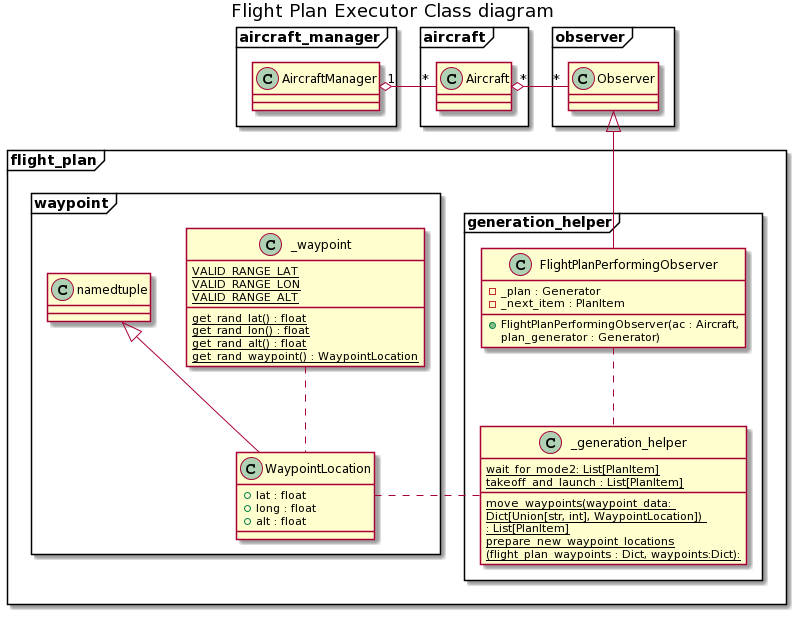
\includegraphics[width=\columnwidth]{UML/flight_plan_executor_class_diagram.png}
    \caption{Flight executor classes}
    \label{fig:flight_plan_executor_class_diagram}
\end{figure}

\begin{landscape}
\begin{figure}
    \centering
    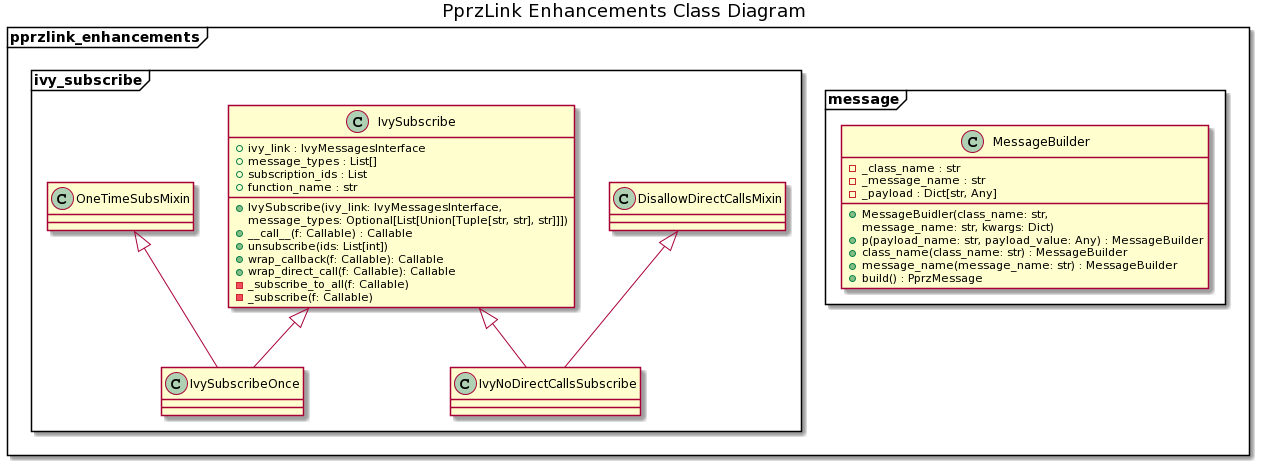
\includegraphics[width=\columnwidth]{UML/pprzlink_enhancements_class_diagram.png}
    \caption{Class diagram for helpers and wrappers for PprzLink library}
    \label{fig:pprzlink_enhancements_class_diagram}
\end{figure}
\end{landscape}

\chapter{Appendix~B: Copyright}\label{appendixb}
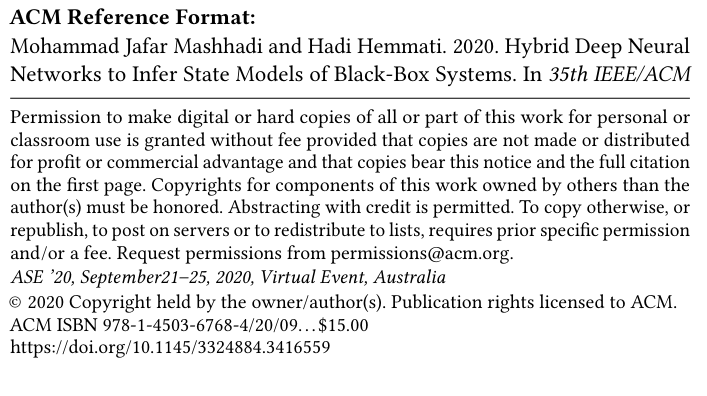
\includegraphics[width=\textwidth]{Copyright.png}
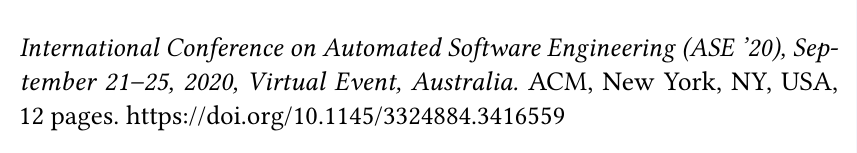
\includegraphics[width=\textwidth]{Copyright2.png}
I, as the author, retained the copyright to the above manuscript while licensing ACM for publication.


\end{document}
